 
\chapter{New insights into AP in myocardial cells}
\label{chap:ap_ventricular_myocyte_localcontrol}

The release of calcium, which is roughly 10x larger than the influx of
calcium, would be supposed to stimulate further CICR, leading to a
re-generative process, or nearly all-or-none release. However,
experimental data have shown that the rate and amount of release from
the SR does not follow the all-or-none behavior, but in a graded
control. This raised the so-called {\it paradoxical of control}. This
paradox of control can be explained by the so-called
{\it local control theory} in which the release of calcium by RyRs via
the CICR was actually the local nanodomains, rather than global
cytosolic calcium. This nanodomain is called {\bf diad subspace} which
is composed of a small cluster of RyRs and DHPR. In the cardiac cells,
there are about 20,000 of such release sites. The global calcium
elevation is thus the result of the recruitment of the calcium release
from these local microdomains. A detail whole-cell models taking into
account all such large amount of number of release sites would
requires high computational demands. 
 


\section{Introduction}
\label{sec:introduction-11}

So far, existing models of cardiac ventricular myocyte haven't
incorporate mechanism of local control of SR $\Ca$ release. Apart from
``common-pool'' models that produce an all-or-none behavior, some can
produce a graded response of $\Ca$ release by formulating $\Ca$
release flux as an explicit function of
$I_\CaL$~\citep{luo1994dmc_b,priebe1998,faber2000,fox2002}. These
phenomenological formulations, however, lack a mechanistic description
of the underlying physiological process. 

A mechanistic model of $\Ca$ dynamics in whole-cell modeling requires
taken into account a realistic number of calcium release units
(CRUs). Depending on cell types (skeletal muscle or ventricular
myocytes), a cluster of IP3Rs and RyRs in a CRU result in 3 distinct
modes of $\Ca$ mobilization:
\begin{enumerate}
\item localized elevation of $\Ca$ due to the activation of a single
  channel, that are referred to as $\Ca$ blips or quarks (depending
  whether the event is driven by IP3R or RyR2)

\item localized elevation of $\Ca$ due to the activation of a cluster
  of channels, referred to as $\Ca$ buffs and sparks, corresponding to
  IP3Rs event and RyR2s event, respectively.


\item global $\Ca$ elevations (oscillations or waves) that is the
  result of the global recruitment of multiple CRUs activation at the
  same time. 
\end{enumerate}
The behavior of each CRU is described in
Chap.~\ref{chap:sparkology-study-ca}.

In addition to the lack of a mechanistic description of the calcium
dynamics in many whole-cell models, others, including those, also
limited in simulating brought about by changes in energetic state of
the myocytes, such as ischemia, where cell metabolism is
compromised. So, it's important to incorporate an energetic model of
energy-dependent channels: Na/K, Na/Ca exchangers and SERCA
pumps. Models for pumps/exchangers are described in
Chap.~\ref{chap:serca-pumps-models} and Chap.~\ref{chap:models-pumps}.



\section{Rice-Jafri-Winslow model (1999)}
\label{sec:rice-jafri-winslow}

JRW model (Sect.~\ref{sec:jafri-rice-winslow}) can reproduce important
frequency-dependent aspects $\Ca$ cycling and {\bf high gain} property, which
refers to the fact that $\Ca$ release from RyR is much higher than $\Ca$ influx.
 However, in this model, $\Ca$ release from RyR doesn't show the {\bf gradeness}
property, i.e. the amount of calcium release is the recruitment of the number of
active calcium release sites (CRUs). The reason is that in JRW model, a single
lumped dyadic subspace is an ensemble average which make the model retaining a
common-pool model and thus cannot introduce gradeness property.

In RJW model, the authors considered explicitly a number of single release
sites. This is indeed the first model that consider ``local-control" mechanism
into modelling. \textcolor{red}{Using stochastic simulation}, each release site
operates as a stochastic functional unit. The local elevation of $\Ca$ at each
release site is known as $\Ca$ sparks.

Based on some experimental data \citep{cannell1995b,cheng1996csc}, under normal
condition, the acitvation of one CRU is not enough to trigger a neighboring CRU
(except under $\Ca$ overload condition), also with very small probability that
they are triggered at the same time. So, they assume all CRUs behave
independently. In addition, under the assumption that $[\Ca]_\myo = 0.1\muM$ and
$[\Ca]_\nsr = 800\muM$ are fixed, then the activation of one CRU is completely
independent from another. So, to avoid computational demand of stochastic
simulation for a large number of CRUs, they run 500 independent trials, each one
simulate simulate a single CRU, and then sum them up to yield the result of a
single cell simulation containing 500 CRUs.

\subsection{Hypothesis analysis}
\label{sec:hypothesis-analysis-6}

In a single diad subspace, the small number of RyR and LCC with random opening
of single channels makes stochastic implementation important.
So, the hypothesis is that \textcolor{red}{ a stochastic implementation is
needed for
  ``gradeness'' behavior with a number of CRUs}.
Based on some experimental data that opening of a single LCCs can trigger $\Ca$
sparks \citep{cannell1995b,lopez-lopez1995}, so RJW modeled a single LCC in the
subspace. Using RYR:LCC $\sim 7.3$ from ~\citep{bers1993rrd}, they assumed 8
RYRs in the cleft space. The system is sufficiently low order to run stochastic
simulation. 

\begin{figure}[hbt]
 \centerline{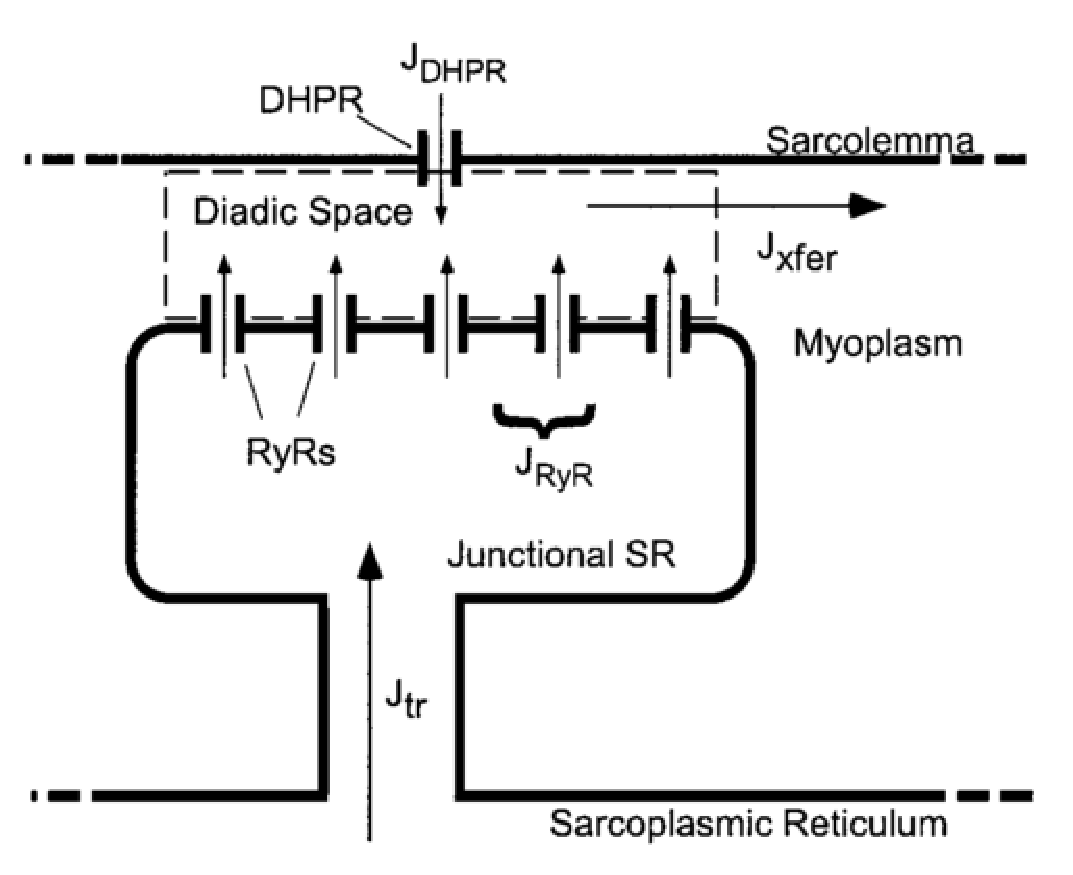
\includegraphics[height=5cm, angle=0]{./images/diadic_subspace.eps}}
\caption{Schematic diagram of a functional release unit model}
\label{fig:diadic_subspace}
\end{figure}

Other assumptions~\citep{rice1999mgg}:
\begin{enumerate}

\item  \textcolor{red}{the whole dyadic subspace is modeled with no spatial
calcium gradient}, Fig.~\ref{fig:diadic_subspace}.

\item each CRU behave independently: ~\citep{cannell1995b,sham1998}
shown that, under normal condition,  $\Ca$ sparks from
one CRU does not spread to the neighboring  ones, except under overload
condition~\citep{cheng1996csc} 

\item based on the above assumption, the activation of multiple CRUs
  leading to global elevation is rared under
  {\it diastolic condition}, so local release doesn't affect
  $[\ca]_\myo$, i.e. myoplasm calcium is fixed $[\Ca]_\myo=0.1\muM$.
  Similarly, the activation of a single SFU doesn't affect the
  $[\ca]_\nsr$. Thus calcium NSR is also assumed constant
  $[\Ca]_\nsr=800\muM$.

  Indeed,
  \textcolor{red}{this is no longer an acceptable assumption since
    when multiple SFU activate at the same time, the $[\ca]_\nsr$
    and $[\ca]_\myo$ are no longer constant}.

\item due to computational demand to simulate thousands of CRUs in a
  cell, thus only a single SFU is simulated at a time, and the
  summation result was collected.  The average after 500 run times,
  can be considered as the ensemble behavior of 500 independent SFU.
\end{enumerate}

\subsubsection{DHPR model}
\label{sec:dhpr-model}


The DHPR is modeled similar to the one in JRW model
(Sect.~\ref{sec:jafri-rice-winslow}) with 5 closed state on the top
($C_0-C_4$), and the mirrored 5 closed state on the bottom
($C_{\text{Ca}0}-C_{\text{Ca}4}$). There are some changes in the
parameters' values.

% The transition rate ($[ms^{-1}]$) for $I_\ca $

\begin{equation}
  \label{eq:1029}
  \begin{split}
    \alpha = 0.4\exp[\frac{V_m+6}{25}] \;\;;
    \beta = 0.05 \exp[-\frac{V_m+6}{29}] \\
    \alpha'=a \times \alpha \;\;;
    \beta' = \frac{\beta}{b} \\
    \gamma = 0.1875 [\ca]_{ss} \;\;;
    \omega = 0.01 \text{ ms}^{-1} \\
    a=2.0 s^{-1} \;\; b = 2.0 s^{-1} \\
    f = 300 \text{ s}^{-1} \;\;;
    g = 2000.0 \text{ s}^{-1} \\
    f' = 5.0 \text{ s}^{-1} \;\;;
    g' = 7000.0 \text{ s}^{-1} \\
  \end{split}
\end{equation}
with $\alpha, \beta$ are $V_m$-dependent activation gates. 

\subsubsection{RYR model}
\label{sec:ryr-model}

To carry out stochastic simulation, a 6-state RyR model based on
~\citep{keizer1998} was used, Fig.~\ref{fig:KeizerSmith_RyR}
(Sect.\ref{sec:Keizer-Smith_98}). This RyR model was created to replicate open
and dwell-times of isolated RyR channels {\it in vitro} and {\it in vivo}, as
well as measured peak and plateau open probabilities with $\Ca$ or cesium
(\ce{Cs^2+}) as the charge carrier. In this study, charge carrier is assumed to
be $\Ca$ only, so all rates depends on $[\Ca]_\ds$ (in the microdomain).
% However, in the original model, some transitions can be dependent upon
% $[\Ca]_\myo$.
% In this study, a modification was made so that all Ca-dependent rate
% transitions use $[\Ca]_\ds$.
Also, the transition rates were modified to match the original description, at
low level of $[\Ca]_\ds$, yet preventing with extremely large transition rates
at high $[\Ca]_\ds$. The reason is that such high rates may be unrealistic, and
for numerical stability, it requires very small time steps, which increase
computational time. To do so, Michaelis-Menten was used to formulate
the saturating of $[\Ca]_\ds$.

% \begin{figure}[hbt]
%   \centerline{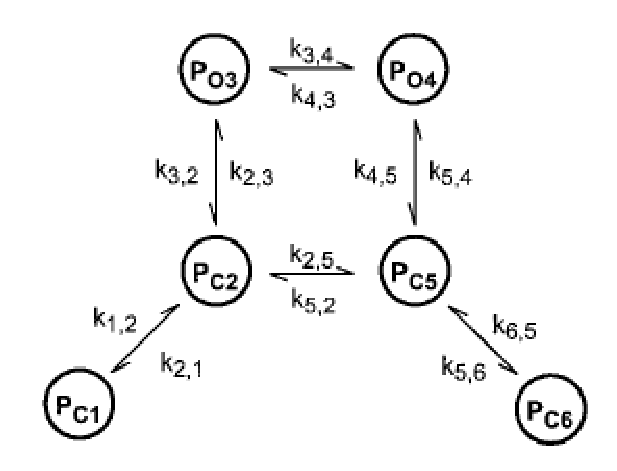
\includegraphics[height=5cm]{./images/KeizerSmith_RyR.eps}}
% \caption{Schematic diagram of a RyR}
% \label{fig:KeizerSmith_RyR}
% \end{figure}

\begin{equation}
  \label{eq:1305}
  \begin{split}
    k_{1,2} &= 3e6 \frac{([\ca]_\ds)^4}{(2.68)^4+([\ca]_\ds)^4} \;\;
    [1/s]\\
    k_{2,1} &=2.5e5 \;\;[1/s] \\
    k_{2,3} &=3e7\frac{([\ca]_\ds)^4}{(2.68)^4+([\ca]_\ds)^4} \;\;
    [1/s]\\
    k_{3,2} &= 9.6e3 \;\; [1/s] \\
    k_{3,4} &= 3e6 \frac{([\ca]_\ds)^4}{(2.68)^4+([\ca]_\ds)^4} \;\;
    [1/s]\\
    k_{4,3} &= 1.3e4 \;\; [1/s]
  \end{split}
\end{equation}

% Further, in this model, adaptation is a property to be assumed
% (\textcolor{red}{In future models, allosteric coupling between RyRs
%   seems to be a better choice}).

\begin{equation}
  \label{eq:1306}
  \begin{split}
    k_{4,5}&= 66.67  \;\; [1/s] \\
    k_{5,4} &= 198 \frac{([\ca]_\ds)^4}{(2.68)^4+([\ca]_\ds)^4} \;\;
    [1/s]\\
    k_{2,5} &= 3e5 \frac{([\ca]_\ds)^4}{(2.68)^4+([\ca]_\ds)^4} \;\;
    [1/s]\\ 
    k_{5,2} &=1.235 \;\; [1/s] \\
    k_{5,6} &= 3e6 \frac{([\ca]_\ds)^4}{(2.68)^4+([\ca]_\ds)^4} \;\;
    [1/s]\\
    k_{6,5} &= 3e6 \;\; [1/s]
  \end{split}
\end{equation}


\subsection{Mathematical model}
\label{sec:mathematical-model-17}

\subsubsection{Ionic currents}
\label{sec:ionic-currents-5}

\begin{enumerate}
\item $I_\CaL$: like JRW-model. However, as there is a single LCCC in the
subspace, (O+O$_\ca$) is substituted by $\DHPR_\open$. Thus, the current form in
eq.\ref{eq:779} becomes the $\Ca$ flux equation
\begin{equation}
\begin{split}
J_\DHPR	 &= %\overline{I_\DHPR}
I_\CaL \frac{\DHPR_\open}{z_\ca F V_\ds} \\
%\overline{I_\DHPR}
 I_\CaL &= \overline{P_\ca } y z^2_\ca \frac{V_mF^2}{RT}
    \frac{0.341[\ca]_o - 0.001\exp[\frac{z_\ca V_mF}{RT}]}{ 1-
      \exp[\frac{z_\ca V_mF}{RT}]}
\end{split}
\end{equation}
with $\DHPR_\open$ is 1 (for LCC in state O or O$_\ca$) and 0 otherwise. $V_\ds$
is the subspace volume. 


\end{enumerate}

\subsubsection{Concentration changes}
\label{sec:conc-chang}

\begin{enumerate}
\item $[\Ca]_\ds$: as there is a single L-type in the subspace, we
  need to modify the formula being used in JRW-model
  \begin{equation}
    \label{eq:542}
    \frac{d[\ca]_\ds}{dt} = \beta_\ds \left( J_\rel 
       - J_{efflux }\frac{V_\myo}{V_\ds} + J_\DHPR 
       %\frac{\DHPR_\open}{z_\ca V_\dsF}I_\ca 
         \right)
  \end{equation}
  with $\DHPR_\open$ is 1 if the DHPR open, and 0 otherwise. 


\item $[\Ca]_\jsr$
  \begin{equation}
    \label{eq:1265}
    \frac{d[\Ca]_\jsr}{dt} = \beta_\jsr( J_\rf - J_\rel\frac{V_\ds}{V_\jsr})
  \end{equation}
\end{enumerate}
\subsubsection{Fluxes}
\label{sec:fluxes-5}

The flux is computed based on the gradient divided by the relaxation
time constant $\tau$ (ms).
\begin{enumerate}
\item $J_\xf$
\begin{equation}
  \label{eq:1027}
  J_\xf = \frac{1}{\tau_\xf}(c_\ds - [\Ca]_\myo)
\end{equation}
with $[\Ca]_\myo=0.1\muM$, $\tau_\ef = 0.0007$ms.
\item $J_\rf$
  \begin{equation}
    \label{eq:1028}
    J_\rf = \frac{1}{\tau_\rf}(c_\nsr-c_\jsr)
  \end{equation}
with $[\Ca]_\nsr=800\muM$, $\tau_\rf=0.005$ms.


\item $J_\rel$: the flux via RyRs (with maximum 8 RyRs opening)
  \begin{equation}
    \label{eq:543}
    J_\rel = \overline{J_\ryr} \sum^8_{i=1}  \RyR^i_\open ([\Ca]_\jsr-[\Ca]_\ds)
  \end{equation}
  with $\overline{J}_\ryr=3960$ [sec$^{-1}$] is the single channel
  permeability to $\Ca$, $\RyR^i_\open$ is 1 if the channel $i$-th is
  open (in state $P_{O3}$ or $P_{O4}$) and 0 otherwise.
\end{enumerate}

\subsubsection{Buffering}
\label{sec:buffering-5}

\begin{enumerate}
\item In the JSR: CSQN is considered, like JRW-model, $\beta_\jsr$ in
  eq.~\eqref{eq:791}.

\item In the subspace: instead of assuming CMDN like JRW-model,
  calcium is assumed to bind to phospholipid anion groups in the 2 places: the
  sarcolemma (SL) and the membrane of the SR (SR). Using fast buffer approximation of \citep{wagner1994erb}
  \begin{equation}
    \label{eq:1266}
    \beta_\ds = \left( 1 +
      \frac{[B]_\SR K_{m,BSR}}{(K_{m,BSR}+[\ca]_\ds)^2} 
      + \frac{[B]_\SL K_{m,BSL}}{(K_{m,BSL}+[\ca]_\ds)^2}\right)^{-1}
  \end{equation}
with $[\B]_\SR=47\muM$ is the total buffer in SR, $[\B]_\SL=1124\muM$
is the total buffer in SL. $K_{m,BSR}=0.87\muM$, and
$K_{m,BSL}=8.7\muM$ based on \citep{smith1998}. 
\end{enumerate}

\subsection{Data analysis}

All simulations use a $V_m$ clamp protocol, running 0.1sec at holding potential
-80 mV to reach the steady state, before a voltage step is applied for 0.2 sec,
and then return to -80 mV. Each trial is repeated 500 times before changing the
voltage step. The voltage step to be used range from -50mV, +50mV with +5mV
increment. 

Using voltage step as +0mV, the result shown 38\% decrease of $[\Ca]_\jsr$
(from 800 to 562$\muM$). In cardiac myocyte, SR retains 35\% of their resting
SR $\Ca$ during a contraction under normal SR load \citep{bassani1995fsr}. 


Effect of adaptation was examined. Slow adaptation produced a larger peak flux
than the control with greater SR unloading. Fast adaptation decrease peak flux,
and also decrease the amount of SR $\Ca$ release.

Mechanisms of SR release termination: local depletion of SR $\Ca$ is assumed to
play a major role, than adaptation. So, what is the main role of adaptation?
e.g. shaping RyR $\Ca$ release, or preventing secondary SR $\Ca$ release from
occuring during an AP - a potential mechanism for early afterdepolarization
(EAD), a proarrhythmogenic condition though to be the basis of torsades de
pointe adn ectopic beating \citep{volders2000}.

For the spark, half-time of decay of spark is measured to be 10 - 40 ms
\citep{santana1996}. $\Ca$ spark amplitude is independent of the duration of LCC
trigger current. However, halting LCC current can stop SR $\Ca$ release
\citep{cleeman1991, wier1994lce}.

During heart failure (HF), a decrease SR $\Ca$ load is observed due to down
regulation of SERCA pump and upregulation of NCX
\citep{ORourke1999,winslow1999}. However, where congestive heart failure (CHF)
can induce change in adaptation has not been confirmed experimentally; and it
can be a potential mechanism of altered DHPR-RyR coupling during CHF.

\section{Greenstein-Winslow (2002) - canine}
\label{sec:greenst-winsl-2002}

Based on the previous model for canine in heart failure, \citep{greenstein2002}
build a whole-cell models incorporating a number of CRUs.

\subsection{Hypothesis analysis}
\label{sec:hypothesis-analysis-18}

This is an extension to the first canine model by~\citep{winslow1999}
(Sect.~\ref{sec:winslow-et-al}), by incorporating a number of dyadic
$\Ca$ release units. The model show that local control is important,
where the LCC inactivation process depend more strongly on local $\Ca$
than on membrane potential, a scenario supported by experimental data.

\subsection{-- CRU}
\label{sec:cru}

The CRU is divided into 4 individual dyad subspace compartments,
arranging into a 2x2 grid. Each dyad subspace (SS) contains a single
LCC, 1 ClCh, and 5 RyRs, Fig.~\ref{fig:Greenstein_CRU}. ClCh is the
$\Ca$-dependent Chlorine current. So, each CRU
has totally 20 RyRs and 4 LCCs, i.e. the stoichiometry is 5:1 for
RyR:LCC which is in agreement with experimental data that one opening
LCC can trigger 4-6 RyRs~\citep{wang2001}.

\begin{figure}[hbt]
  \centerline{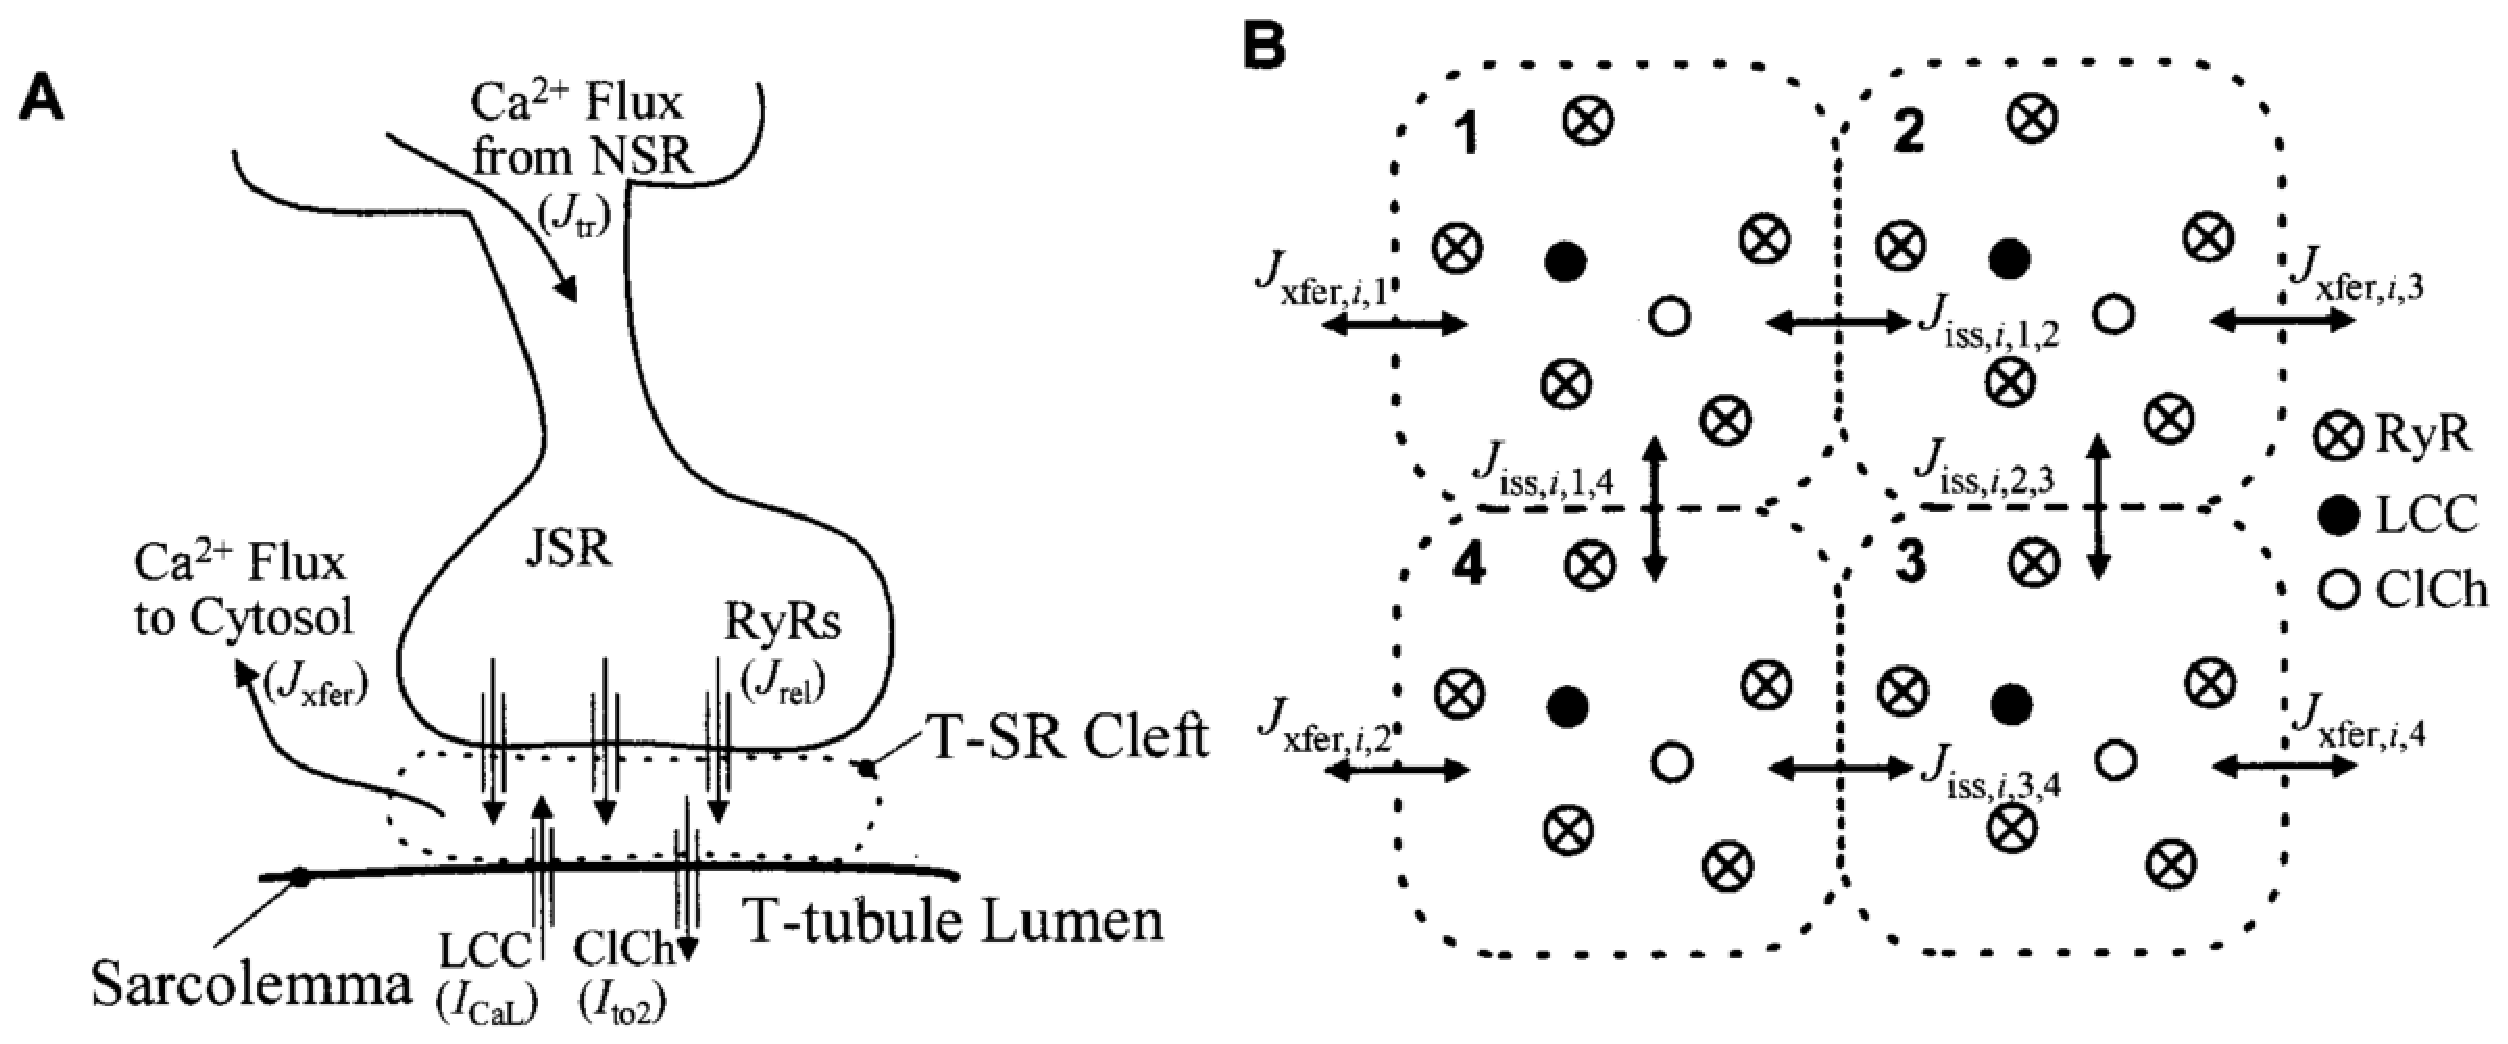
\includegraphics[height=5cm,
    angle=0]{./images/Greenstein_2002_CRU.eps}}
  \caption{A schematic diagram of a CRU, divided into 4 dyad
    subcompartment. $J_{\iss,i,j}$ is the passive diffusion of $\Ca$
    between dyads in a single CRU; $J_{\xfer,i,j}$ is the passive
    diffusion of $\Ca$ from the dyad to the cytosol}
\label{fig:Greenstein_CRU}
\end{figure}

$\Ca$ in a single compartment is assumed to be uniform, and can
diffuse passively to neighboring dyad compartment within the same
CRU; with a rate 10-fold slower compare to the flow from the subspace
to the cytosol. 
\begin{itemize}
\item The inter-subspace transfer rate $v_\iss = 20$ ms$^{-1}$, which
  corresponds to diffusion coefficient of $\sim 330\mu$m$^2$.s$^{-1}$
  when the assumed height of the model subspace is 12nm. This is
  similar to estimates from experiments~\citep{soeller1997}.

\item The purpose of dividing into 4 dyad compartment is for easy of
  computational handling, and it's assumed that when one LCC activate, it can
  trigger all 5 RyRs. However, using this method, it lacks the capability that
  RyRs in one dyad may also trigger the adjacent RyRs in the neighboring dyad.
\end{itemize}

\textcolor{red}{NEW: The calcium-dependent transient outward} $\ce{Cl-}$
  current $I_\text{to2}$ in also included as part of the CRU.
  This has not been included in the first canine whole-cell model by~\citep{winslow1999}. However,
  for simplicity,
\textcolor{red}{the concentration of intracellular} $[\Cl]$ is assumed
  to be constant.

\label{sec:Cl-channel}
The $\ce{Cl-}$ channel (ClCh) has low $\Ca$ binding affinity, $K_{d,\ClCh}\sim
150\mu$M. $I_\text{to2}$ is abolished in the presence of caffeine. The density
of these channels is in the range 3-4$\mu$m$^{-2}$~\citep{collier1999}, similar
to density of active LCC (2-5$\mu$m$^{-2}$). So, they assume a single ClCh per a
dyad subspace. $I_\text{to2}$ is modeled using simple 2-state model,
Fig.~\ref{fig:Greenstein_ClCh}, with unitary conductance is 8.2pS (measured at
the range -80mV to -20mV)~\citep{collier1999}.

% \begin{equation}
%   \label{eq:1323}
%   I_{to2} = \frac{}{} \sum^{N_\SFU}_j \sum^4_i I_{\ClCh,i,j}
% \end{equation}
\begin{figure}[hbt]
  \centerline{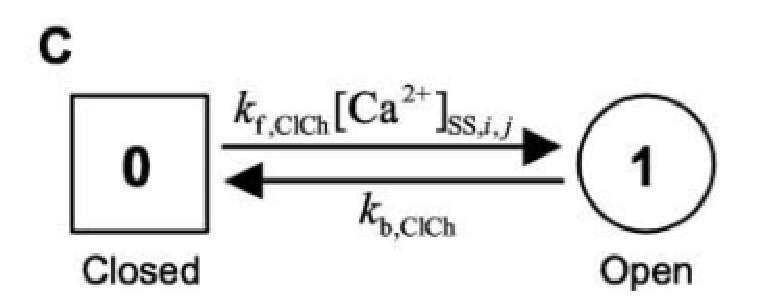
\includegraphics[height=2cm,
    angle=0]{./images/Greenstein_ClCh.eps}}
\caption{2-state ClCh channel}
\label{fig:Greenstein_ClCh}
\end{figure}

\subsection{-- $I_{to2}$ current}

$I_{to2}$ is given in eq.~\eqref{eq:1330}
\begin{itemize}
\item $k_{f,\ClCh}=13.3156$[1/(mM.sec)]
\item $k_{b,\ClCh}=2.0$[1/(sec)]

\item $K_{d,\ClCh}=0.1502$mM the dissociation constant of ClCh for
  $\Ca$.
\end{itemize}


\subsection{-- LCC}
\label{sec:lcc}

See Sect.\ref{sec:LCC_greenstein2002}.

\subsection{-- RyR}

The model for RyR is based on~\citep{rice1999mgg}
(Sect.~\ref{sec:rice-jafri-winslow}), a modification from~\citep{keizer1998}, in
which adaptation is a distinct feature. However, as the data is not enough to
constraint RyR model parameters, the property of adaptation is not retained. 
Besides, $\Ca$-dependent of state transition was modified based on the
assumption that 4 ions must bind to the channel before it can
open~\citep{zahradnikova1999}. So, from 6-state RyR model, a 4-state RyR model
was derived and used (Sect.\ref{sec:greenstein_winslow_RyR}).

 
\subsection{-- Buffering}
\label{sec:buffering-3}
\begin{enumerate}
\item Buffering in subspace is assumed to be
  rapid~\citep{wagner1994erb}, with the buffers are (immobile)
  phospholipid anion groups on both SR and sarcolemmal membranes.

\item Buffering for JSR $\Ca$ are assumed to be $\Ca$-calsequestrin
  binding~\citep{shannon2000rms}.

\end{enumerate}
\subsection{-- Other ionic currents}
\label{sec:other-ionic-currents}

There are some changes in ionic currents formulation
\begin{enumerate}
\item $I_\text{to1}$ is modeled based on~\citep{greenstein2000} with
  new parameters' values: $G_{Kv4.3} = 0.1389$mS/$\mu$F, and the
  permeability $P_{Kv4.3}=1.989e-3\mu$m/s.

  Previous model predicted: [the reduce in density lead to (1) modest
  shortening of APD, (2) reduce the depth of phase 1 AP notch, (3)
  reducing the peak of $I_\CaL$]

\item $I_\Kr$ is modeled based on~\citep{mazhari2001}
\item SERCA pump is modeled using~\citep{shannon2000rms} which
  accounts both forward and reverse mode. 

\item other ionic currents are rescaled to preserve cytosolic ionic
  concentration and AP shape.
\end{enumerate}

\subsection{Mathematical analysis}
\label{sec:math-analys-2}

\subsection{-- Ionic currents}
\label{sec:ionic-currents-9}

\begin{framed}
  So, to normalized the whole-cell current by whole-cell capacitance,
  to avoid the variance in $\Csa$ between cells, we need to multiply
  with $\frac{1}{\Csa}$; with $\Csa=153.4$pF = $A_{cap}.\Csc$ with
  $\Csc=1\mu$F/cm$^2$.
\end{framed}

\begin{enumerate}
\item Whole-cell $\Ca$ current~\citep{handrock1998}
  \begin{equation}
    \label{eq:1324}
    I_\CaL = N_\act . i_\CaL . p_o 
  \end{equation}
  with $N_\LCC$ is the number of LCCs in the cell, $i_\CaL$ is single
  channel current, $p_o$ is open probability.

  The current passing through a single channel is formulated using
  constant field theory (GHK equation)
  \begin{equation}
    \label{eq:1334}
    \begin{split}
      I_{\CaL,i,j} = \isopen(\LCC_{i,j},y_{i,j}) P_\CaL \times z_\ca^2
      \frac{V_mF^2}{RT} \\
      \frac{0.341[\Ca]_o-\exp(z_\ca V_mF/(RT))
        [\Ca]_\myo}{1-\exp(z_\ca V_mF/(RT))}
    \end{split}
  \end{equation}
  with $\isopen(\cdot)$ is 1 when the LCC channel occupies state O or
  O$_\ca$, and is not $V_m$-inactivated (i.e. $y_{ij}=1$), and takes
  on 0 otherwise. $P_\CaL=$

  The normalized current ($\mu$A/pF)
  \begin{equation}
    \label{eq:1335}
    I_\CaL = \frac{1}{\Csa}\frac{N_\CRU}{N_s} \sum^{N_s} \sum^4 I_{\LCC,i,j}
  \end{equation}



\item Whole-cell $I_{to2}$
  \begin{equation}
    \label{eq:1331}
    I_{to2} = \frac{1}{\Csa} \sum^{N_\CRU}_i \sum^4_j I_{\ClCh, i, j}
  \end{equation}
  However, the number of CRU to be simulated $N_s$ is typically smaller than
  the those in the full model, so to rescale to the true number, an
  approximation is given
  \begin{equation}
    \label{eq:1330}
    I_{to2} =\frac{1}{\Csa} \frac{N_\CRU}{N_s}\sum^{N_s}_i \sum^4_j I_{\ClCh, i, j}
  \end{equation}
  with single-channel current is modeled using constant-field theory
  (unit is [pA])
\begin{equation}
  \label{eq:1332}
  I_{\ClCh,i,j} = \isopen(\ClCh_{i,j}) P_{to2} z_\Cl^2
  \frac{V_mF^2}{RT} \frac{[\Cl]_o-[\Cl]_i \exp(-z_\k
    \frac{V_mF}{RT})}{1-\exp(-z_\k \frac{V_mF}{RT})}
\end{equation}
with $z_\Cl=1$, $P_{to2} = 2.65e-3\mu$m$^3$/sec ($\Ca$-dependent $\Cl$
channel permeability to $\Cl$) .
\end{enumerate}

\subsection{-- Fluxes}
\label{sec:fluxes-9}

\begin{enumerate}
\item From each subspace compartment, there are flux of calcium
  diffusing to adjacent subspace compartment $J_{\iss,i,j,k}$ (from
  $j$-th to $k$-th subcompartment in the $i$-th CRU), and flux of
  calcium diffusing to the bulk myoplasm $J_{\ef,i,j}$ (or $J_\xfer$)
  (from the $j$-th subcompartment of the $i$-th CRU to the cytosol).
  \begin{equation}
    \label{eq:1325}
    \begin{split}
      J_{\ef,i,j} = v_\ef( [\Ca]_{\ds,i,j}-[\Ca]_\myo)\\
      J_{\iss,i,j,k} = v_\iss ([\Ca]_{\ds,i,j}-[\Ca]_{\ds,i,k} \\
    \end{split}
  \end{equation}
with $v_\ef = 200$[1/sec], $v_\iss = 20$ [1/sec]

\item Each CRU receives passive calcium diffusion from the network SR
  $J_{\rf,i}$ (or $J_\tr$) (the $i$-th CRU receive the refill)
  \begin{equation}
    \label{eq:1326}
    J_{\rf,i} = v_\rf ([\Ca]_\nsr - [\Ca]_{\jsr,i})
  \end{equation}
with $v_\rf = 0.333$ [1/sec]. So, the total flux from NSR to all CRUs
is
\begin{equation}
  \label{eq:1327}
  J_\rf = \sum^{N_\CRU}_{i=1} J_{\rf,i}
\end{equation}
However, as we typically simulated with a smaller amount of CRU, say
$N_s$ rather than the number of CRU in the full model, say
$N_\CRU$. So, we use the formula
\begin{equation}
  \label{eq:1328}
  J_\rf \approx \frac{N_\CRU}{N_s}\sum^{N_s}J_{\rf,i}
\end{equation}
\end{enumerate}

\subsection{-- Ion concentrations}

Intracellular $[\Na]_i$, $[\K]_i$, NSR $\Ca$ and cytosolic $\Ca$ are dynamics. 

\subsection{Numerical solving}
\label{sec:numerical-solving-2}

All state variables ($V_m$) and ionic currents are added a stochastic
noise as the result of the Monte-Carlo simulation. 

The time progression of states for single channels within each CRU is calculated
individually. It means that the Monte Carlo simulation of channel gating are
performed independently between different channels: RyR, LCC, ClCh; so that the
time evolution can be different. The choice of next state for individual
channels are determined by using a set of random variables. 

Time steps for simulation are adaptive, with sufficiently small, to update local
variables, i.e. $[\Ca]_{\ds,i,j},...$. A larger time step is used to update the
global variables, e.g. $[\Ca]_\myo, V_m...$. It means that these global
variables are less often to be updated. This will reduce the computational
efforts. Between two global update, when local updates is required,
the global variables are assume unchanged. 

The majority of computational time is spent on stochastic simulation
for CRUs, which is highly parallelizable under the assumption that
CRUs behave independently. The simulation run on SGI Power Challenge symmetric
multiprocessing  computer configured with 12 R10,000 processors and 1GB memory. 

A simulation is typically with a smaller number of CRUs, and the result are
rescaled (approximation) to the true number of CRUs in the cell. 

\subsection{Data analysis}
\label{sec:data-analysis-1}

Even though the number of LCC were chosen as with NSFU = 12,500 CRUs,
the number of CRUs being used in the simulation is lower, about
10x. This takes $\sim 40$ min for a single second simulation on 10
SGI Power Challenge R10,000 processors with 1GB RAM.

In older models~\citep{jafri1998cad, luo1994dmc_b}, $I_\CaL$ has a
strong $V_m$-dependent inactivation, and relatively weak
$\Ca$-mediated inactivation. This, however, is opposite the local
control model, with $\sim 35\%$ of LCC are $V_m$-dependent and $\sim
75\%$ are $\Ca$-dependent inactivation. 

Cytosolic $[\Ca]_i$ transient reaches the peak at 0.75$\mu$M, while
calcium in the subspace reaches $\sim 11\mu$M on average, and
equilibrate to near cytosolic level rapidly, within 100-150ms. In
essence, the model predicted subspace calcium concentration is
$>20$-fold higher than cytosolic concentration during membrane
depolarization. 

The result, Fig.~\ref{fig:Greenstein_fig9}, shown that $I_\CaL$ peaks
at $\sim 4.7$pA/pF, with a sustained component (the tailing part)
of $\sim 0.7$pA/pF that lasts for nearly the entire AP. The peak
$I_{to2}$ is $\sim 0.6$pA/pF. 

\begin{figure}[hbt]
  \centerline{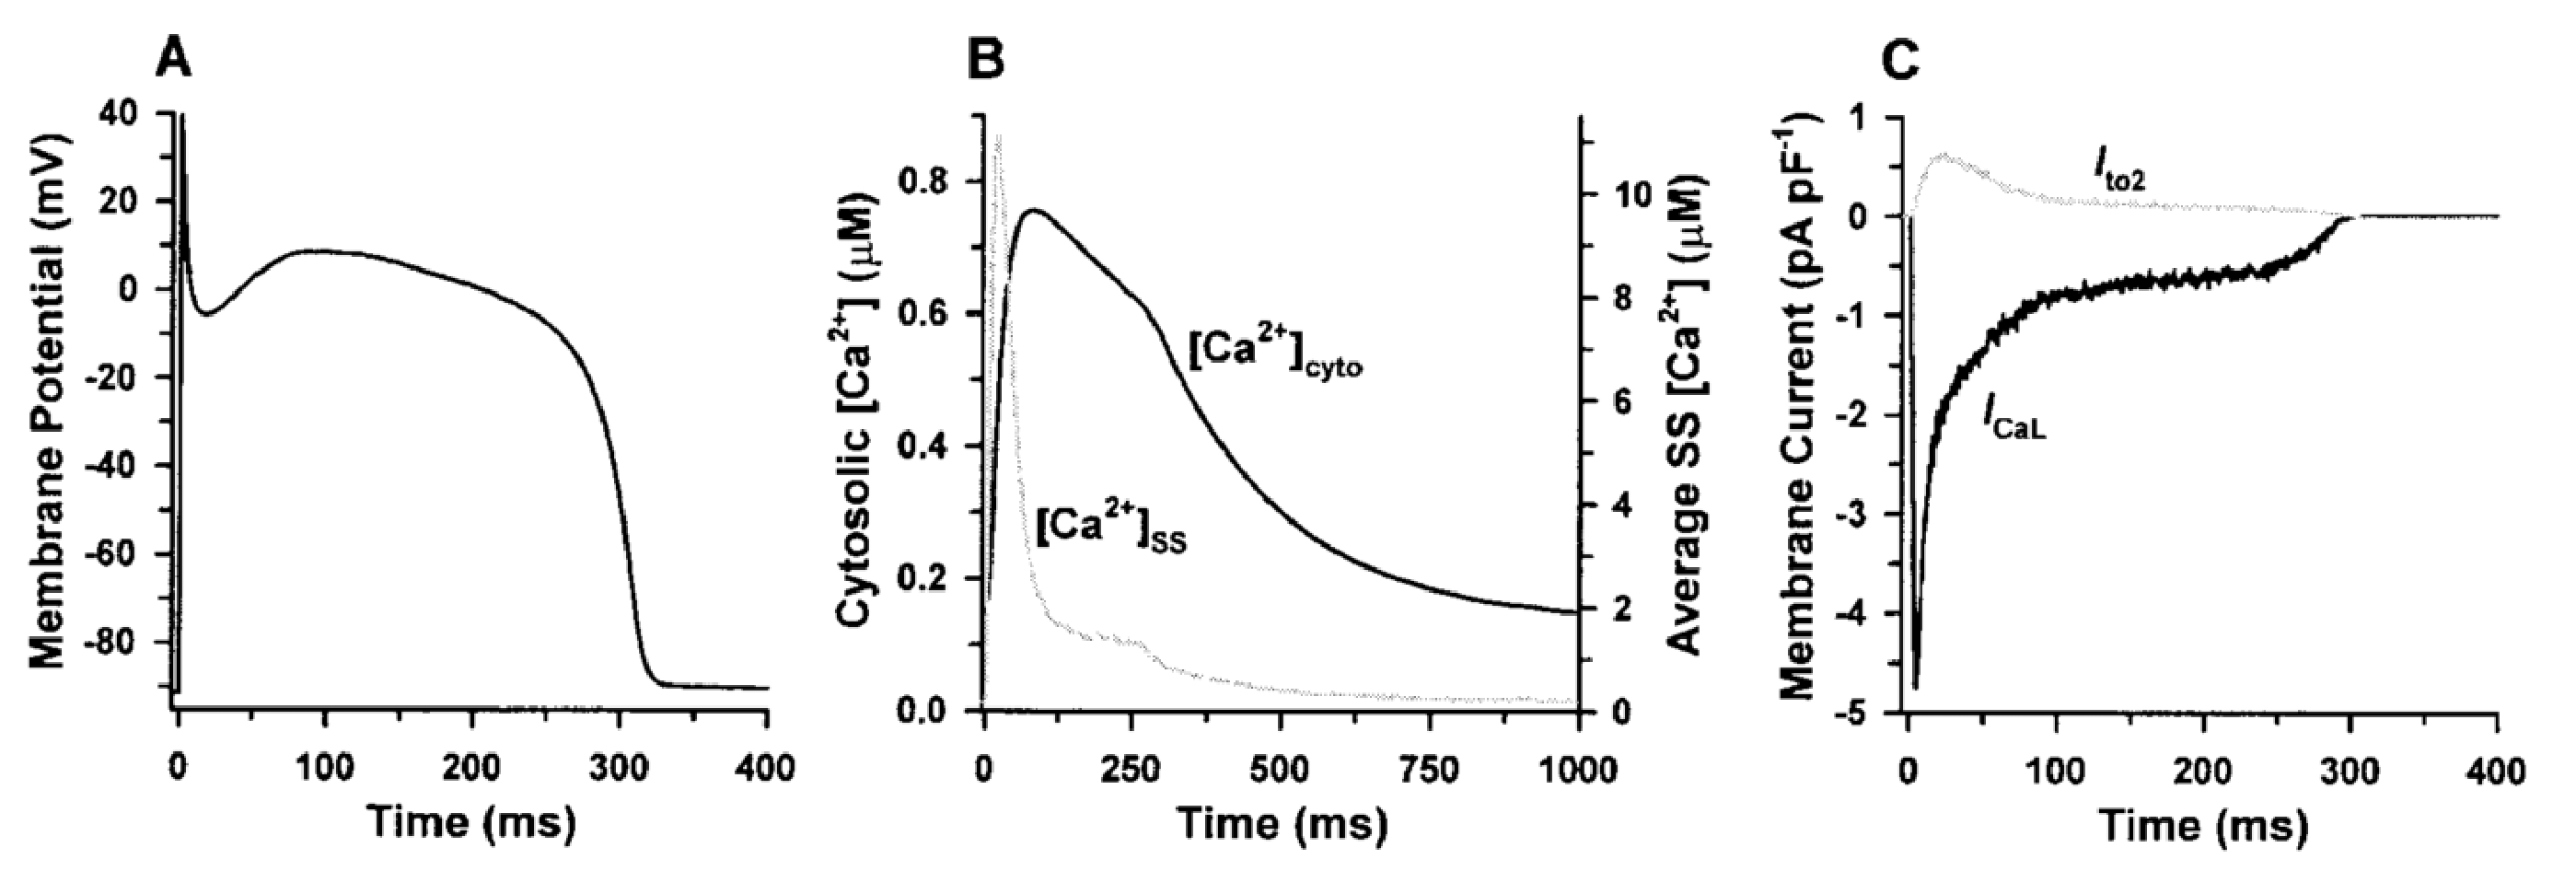
\includegraphics[height=5cm,
    angle=0]{./images/Greenstein_fig9.eps}}
  \caption{AP, $[\Ca]$ transient (cytosolic, and subspace), and
    membrane current}
\label{fig:Greenstein_fig9}
\end{figure}


Under normal condition, APD is about 315ms. The peak flux via RyR is
$\sim 0.8$ mmol/(L-cytosol.sec)


\section{Wang-\ldots-Levine (2005)}
\label{sec:Wang-Levine2005}

Model for RyR is discussed in Sect.\ref{sec:wang-levine2005_RYR}. Here, it's
assumed that FKBP only couple subunits in the same RyR tetramer. There are
evidences that FKBP also couple neighboring RyRs \citep{marx1998, marx2001}. 
Model for LCC is used from \citep{iyer2004} with 13 states (11 voltage and
calcium-dependent states; and 2 voltage-dependent inactivation states)
(Sect.\ref{sec:Iyer-Winslow2004}). 

EC-coupling gain is defined as 
\begin{equation}
\text{Gain} = \frac{J_{\ryr,\max}-J_{\ryr,\rest}}{J_{\dhpr,\max}}
\end{equation}
with the fluxes are maximal values during EC-coupling; and $J_{\ryr,\rest}$ is
the release of $\Ca$ in the absence of opening LCC (resting condition). 

There are two scenarios: (1) the simple model is when $[\Ca]_\nsr$ is constant
and a single CRU is triggered; (2) the full model, when they uses 100 CRUs, and
calcium both in myoplasm and network SR are treated as dynamical variables.



\subsection{Mathematical model}

The current through L-type at conducting
states is
\begin{equation}
I_\dhpr = P_\ca z_\ca^2 FV_m \times (F/RT) \frac{[\Ca]_\ds \times
e^{z_\ca.V_m(F/RT)} - 0.341[\Ca]_o }{e^{z_\ca.V_m(F/RT)}-1.0}
\end{equation}
with $N_{\dhpr,o}$ opening channels, the total flux is 
\begin{equation}
J_\dhpr = - \frac{N_{\dhpr,o}I_\dhpr}{z_\ca.F.V_\ds}
\end{equation}

Dynamics of calcium in the subspace
\begin{equation}
\frac{d[\Ca]_\ds}{dt} = J_\ryr + J_\dhpr + J_\buf - J_\ef
\end{equation}
with 
\begin{equation}
J_\ef = \frac{[\Ca]_\ds	- [\Ca]_\myo}{\tau_\ef}
\end{equation}
The binding of calcium to buffers in the subspace use the formula from
\citep{sobie2002tcas} (Sect.\ref{sec:sobie2002_jafri}) : 
\ce{Ca + B <=>[k_{j,on}][k_{j,off}] CaB}
\begin{equation}
J_\buf = - \sum_j \left( k_{j,on}[\Ca]_\ds\left([\B]_j-[\CaB_j] \right) -
k_{j,off}[\CaB_j] \right)
\end{equation}
using 3 buffers $B_j$ ($j=1,2,3$): Calmodulin, SR membrane buffers, and
sarcolemmal membrane buffers of constant concentration.


Rapid buffering is assumed in the jSR area, between calcium and Calsequestrin,
based on \citep{greenstein2002} (Sect.\ref{sec:greenst-winsl-2002}). So, the
dynamics of calcium in the jSR is
\begin{equation}
\frac{d[\Ca]_\jsr}{dt} = \beta_\jsr\left( -\frac{V_\ds}{V_\jsr}J_\ryr +
J_\rf \right)
\end{equation}
with 
\begin{equation}
J_\rf = \frac{[\Ca]_\nsr - [\Ca]_jsr}{\tau_\rf}
\end{equation}


\subsection{Numerical analysis}

Using continuous time discrete-state Markov-chain process to describe the
channels, at each time step, a pseudo-random number is generated, for each
channel, to determine how its state should be updated, based on the current rate
equations. 

The time step is chosen as $\Delta t=10^{-5}$ (sec). Euler method is used. 

The data are collected based on triggering CRUs (once every second), by clamping
$V_m$ from holding potential -80mV to a higher potential (0mV) for a duration of
100ms. 

\subsection{Data analysis}

The EC-coupling gain, with $s=0.5$, is shown in Fig.\ref{fig:Wang2005_ECgain}.
The authors claimed that the curve is insensitive to $s$. The result showed that
gain is a monotonically decreasing function of $V_m$.

\begin{figure}[hbt]
  \centerline{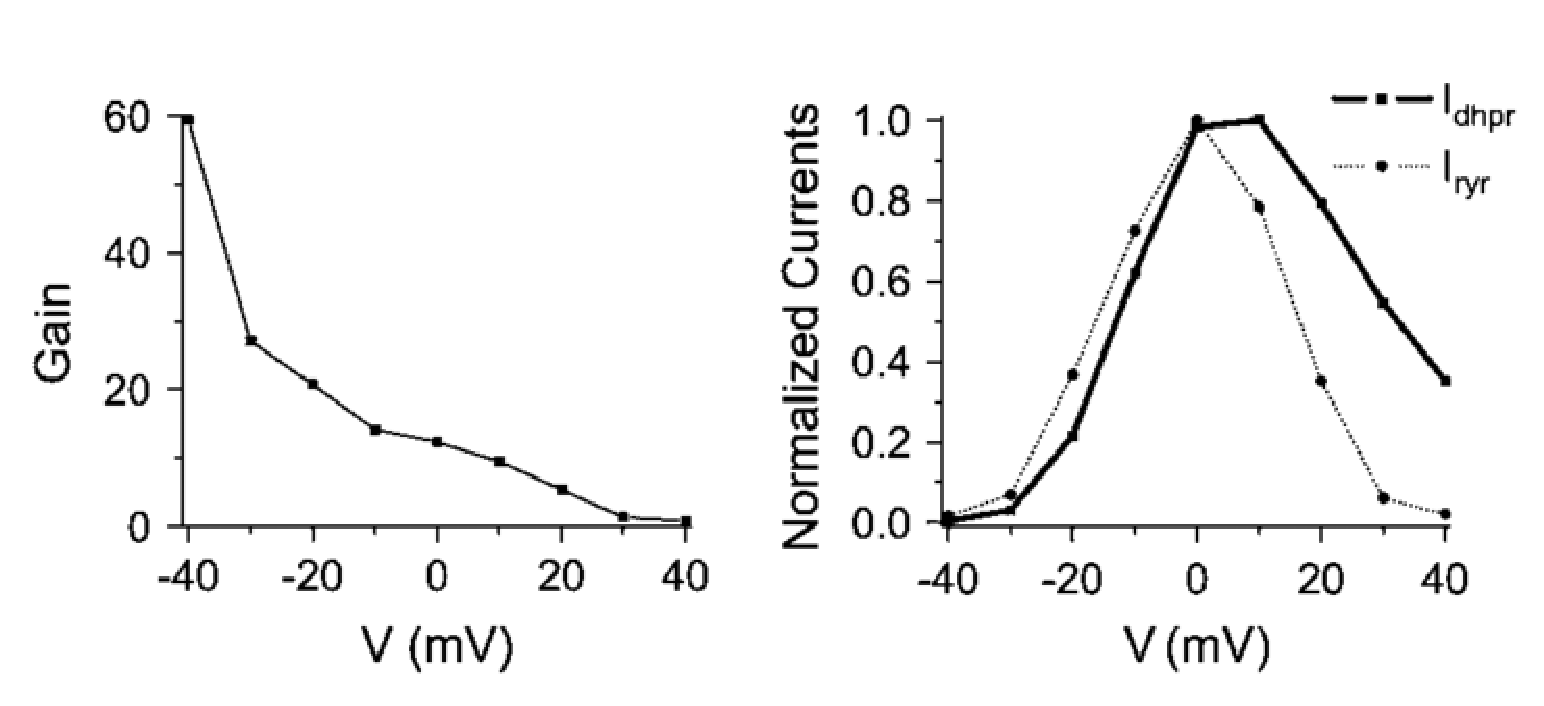
\includegraphics[height=3.5cm]{./images/Wang2005_ECgain.eps}}
\caption{EC-coupling gain with $s=0.5$ }
\label{fig:Wang2005_ECgain}
\end{figure}

When studying the dynamics of $[\Ca]_\ds$ using different value of the
cooperativity value $s$, they realized that the decay rate is larger and peak
calcium is higher when $s$ is increased. However, the peak calcium reaches the
maximum value at $s^* \sim 0.4$. This is also the value of $s$ at which the
calcium release is peaked, i.e. the gain function of $s$ is highest at $s=s^*$,
Fig.\ref{fig:Wang2005_couplestrength}.

\begin{figure}[hbt]
  \centerline{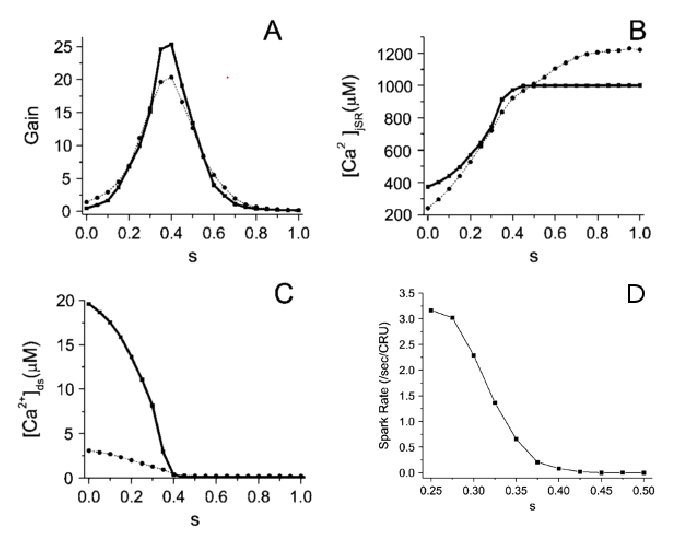
\includegraphics[height=5cm]{./images/Wang2005_couplestrength.eps}}
  \caption{Gain, resting $[\Ca]_\jsr$, $[\Ca]_\ds$ and the spontaneous spark
  rate as the function of couple strength $s$. Thick line = result when simple
  model is used. Thin line = full model is used}
\label{fig:Wang2005_couplestrength}
\end{figure}


Studying a single CRU, it's showed that spontaneous frequency (per second per
CRU) increased with decreasing value of $s$,
Fig.\ref{fig:Wang2005_couplestrength}(D).

Limitation: the model cannot investigate the fight-or-flight response: during
which $\beta-$adrenergic pathway is stimulated and PKA level is increased.
Here, the net result is an increase in EC-coupling gain and cardiac output
(Sect.\ref{sec:cardiac-output}) \citep{wehrens2003af}. The signalling pathways
not only affect RyRs, but also LCC channel and calcium-uptake through SERCA
pump. Such mechanism has not been incorporated into the model.

So far, there is no developed quantitative link between FKBP concentration and
the coupling strength $s$. This would requires direct measurement of the
gating mechanism while varying KFBP concentration. Also, a spatially extended
model that include cooperativity between neighboring RyRs, coupled to a detailed
electrophysiological model need to be developed. 


\section{Greenstein-Hinch-Winslow (2006)}
\label{sec:greenst-hinch-winsl}

~\citep{greenstein2006} proposed a simplified deterministic model
based on ~\citep{greenstein2002} (Sect.~\ref{sec:greenst-winsl-2002}).
In this model, each CRU has a single LCC and a single RyR. Then the global state
of a CRU is built by combining the state space of single LCC and that of single
RyR. This joint behavior can then be described by a Markov model, referred to as
coupled LCC-RyR gating models. 

\subsection{LCC model}

A simplified version of JRW model \citep{jafri1998cad}
(Sect.\ref{sec:LCC_Jafri1998}) was used.
\begin{enumerate}
  \item state O$_\ca$ is dropped. 
  \item state C0, C1, C2 and C3 and I0, I1, I2, I3 are combined to make a
  5-state Markov model. The effect of this change is a minor alteration in the
  activation kinetics of LCC.
\end{enumerate}
So, in each mode, there are 2 closed state. Totally, we have 5 states.
This model can be simplified into 3-state by assuming the transition between C1
and C2; I1 and I2 are rapid relative to transition rate between the two modes. 
$V_m$-dependent inactivation has not been considered.

\begin{figure}[hbt]
  \centerline{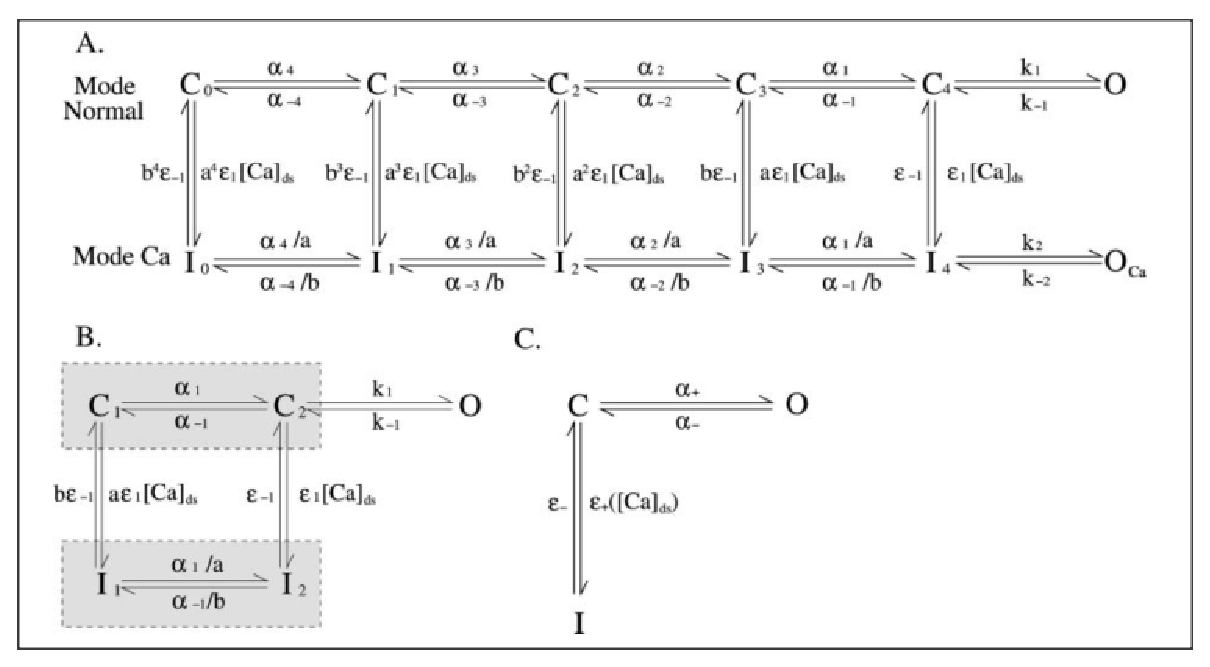
\includegraphics[height=5cm,
    angle=0]{./images/greenstein_LCC_06.eps}}
\caption{Reduced LCC models}
\label{fig:greenstein_LCC_06}
\end{figure}

\subsection{RyR model}

Here, RyR inactivation is the primary mechanism of termination SR $\Ca$ release.
Based on scheme 6 of \citep{stern1999lcm}, with the addition of modal gating
betweens state C and O. Then using rapid equilibrium assumption, C1 and C2 are
combined; I1 and I2 are combined. 

\begin{figure}[hbt]
  \centerline{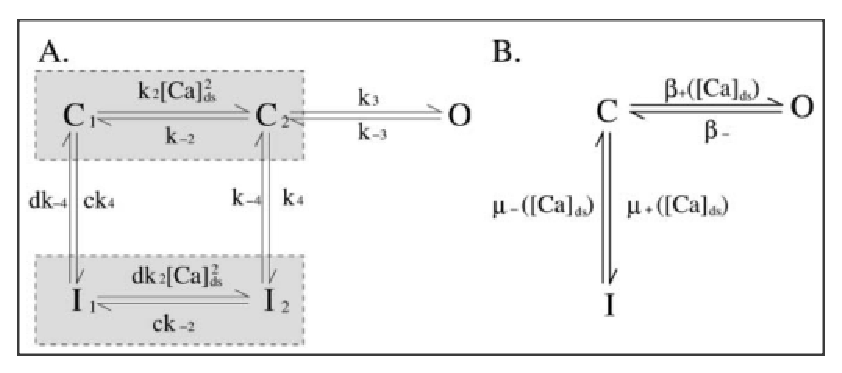
\includegraphics[height=5cm,
    angle=0]{./images/greenstein_RyR_06.eps}}
\caption{Reduced RyR models}
\label{fig:greenstein_RyR_06}
\end{figure}

\subsection{CRU model}

The separate JSR has not been included in the model based on the fact that some
study suggest JSR is in quasi-equilibrium with NSR \citep{shannon2003}.	

Combining a 3-state RyR with 3-state LCC, a 9-state CRU model is built. 

\begin{figure}[hbt]
  \centerline{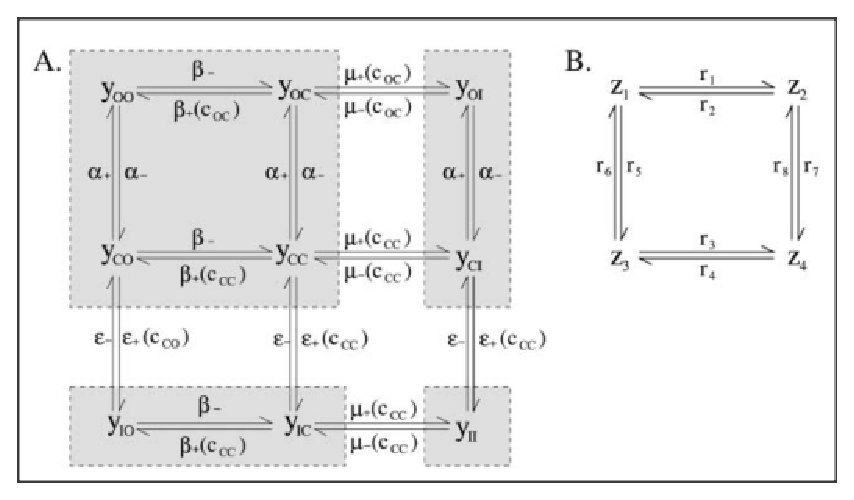
\includegraphics[height=5cm,
    angle=0]{./images/greenstein_CRU_06.eps}}
\caption{Coupled LCC-RyR model}
\label{fig:greenstein_CRU_06}
\end{figure}


\subsection{Numerical analysis}

The model was solved using variable-step fourth-order Runge-Kutta integration
algorithm on a PC with 2GHz processor and 512 MB RAM.





\section{Williams et al. (2007)}
\label{sec:williams-et-al}


% There have been many mathematical models developed to test hypotheses
% about heart cell function and, hopefully, predict underlying
% mechanism. The numerical approach to these models is deterministic,
% which ignore molecular fluctuations and assume
% {\it isopotential cell}. In other words, such methods claim that

The claim for using deterministic method in cardiac cell modeling is
that ``even though the kinetics of individual channels is stochastic,
with large enough number of ion channels, experiences the same
voltage, identical rate constants can be applied and thus, the average
behavior is deterministic''. However, as proven in RJW model
(Sect.~\ref{sec:rice-jafri-winslow}), such approach is not adequate
for simulating CICR during ECC.

The main point is that the elementary event of of ECC is the local
transient of \ce{Ca^2+} - known as \ce{Ca^2+} spark - at which the
number of LCC and RyR is small. As a result, stochastic behavior is
expected, and thus stochastic simulation is important.


\subsection{Hypothesis analysis}
\label{sec:hypothesis-analysis-11}

A complete description of CICR should takes into account a realistic
number of CRU, $N\sim 20,000$, each with 1-10 DHPR and a larger
cluster of RyR2s (30-300). ~\citep{williams2007pda} developed a
computational whole-cell model using stochastic simulation, and
derived an efficient computational method using probability density
approach, in replacement for Monte Carlo simulation.  


Typically, each channel is described by a Markov-chain model with 2 to
tens of states.  Some models indicated that the sparks behave in an
all-or-none manner, so
\textcolor{red}{~\citep{williams2007pda} assume each CRU has a single RyR
  ``megachannel'', and one L-type channel}.
Essentially, each CRU has 1 LCC and 1 megachannel RyR.  In addition,
to avoid the complexity as of a minimal model, there are certain a
number of assumptions:
\begin{enumerate}
\item Each CRU has 2 restricted compartments: the dyadic subspace (ds)
  and junctional-SR.
\item Two-state DHPR model and two-state RyR model

\item Only $V_m$-dependent activation is considered in L-type $\Ca$
  channel, i.e. it ignores the voltage- and \ce{Ca^2+}-dependent of
  the inactivation rate $k^-_{dhpr}$. The judgement of this claim is
  that calcium doesn't affect much to the triggering of CICR during
  whole-cell $V_m$-clamp which is the focus of the study. 
  \begin{equation}
    \label{eq:83}
    \ce{C  <=>[k^+_\dhpr(V_m)][k^-_\dhpr] O}
  \end{equation}
with 
\begin{equation}
  \label{eq:1349}
  k^+_\dhpr = \overline{k^+}_\dhpr \frac{\exp(\frac{V_m-V^\theta_\dhpr}{\sigma_\dhpr})}{1+\exp(\frac{V_m-V^\theta_\dhpr}{\sigma_\dhpr})}
\end{equation}
where $V^\theta_\dhpr=-10$ mV is the activation threshold,
$\sigma_\dhpr=6.24$ mV is the activation parameter, and
$\overline{k^+}_\dhpr=556$ [1/sec].

The constant deactivation rate $k^-_\dhpr=5000$ [1/sec] is chosen to
set the mean open time 0.2ms and maximum open probability
$P_{o(\max)}=0.1$.

\item Activation of RyR megachannel is assumed to be
  $[\Ca]_\ds$-dependent and lumenal calcium $[\Ca]_\jsr$ dependent.
  \begin{equation}
    \label{eq:1336}
    \ce{ C <=>[k^+_\ryr(c^\ii_\ds,c^\ii_\jsr)][k^-_\ryr] O}
  \end{equation}
with activation is a sigmoidal function of the $[\Ca]_\ds$
\begin{equation}
  \label{eq:1347}
  k^+_\ryr = \overline{k^+}_\ryr \frac{([\Ca]_\ds^\ii)^4}{(K_{m,\ryr})^4+([\Ca]_\ds^\ii)^4}
\end{equation}
with maximum rate of RyR opening $\overline{k^+}_\ryr=2000$ [1/sec], and
the influence of junctional SR $[\Ca]$ is to make half-maximal
activation a decreasing function of $[\Ca]_\jsr$.
\begin{equation}
  \label{eq:1348}
  K_{m,\ryr} = K^\max_\ryr - \alpha_\ryr [\Ca]_\jsr^\ii
\end{equation}
where $K^\max_\ryr = 7.4\mu$M is maximum binding constant for RyR,
$\alpha_\ryr = 0.0024$ [unitless] is coefficient or RyR luminal
regulation. 

NOTE: The depletion of $[\Ca]_\jsr$ will render the CRU refractory to
activation after release terminate. 

\item All-or-none behavior of DHPR and RyR channels $==>$ CaRU is
  modelled as a 4-state release site, Fig.~\ref{fig:Blair_CRU}.
\end{enumerate}

\begin{figure}[hbt]
  \centerline{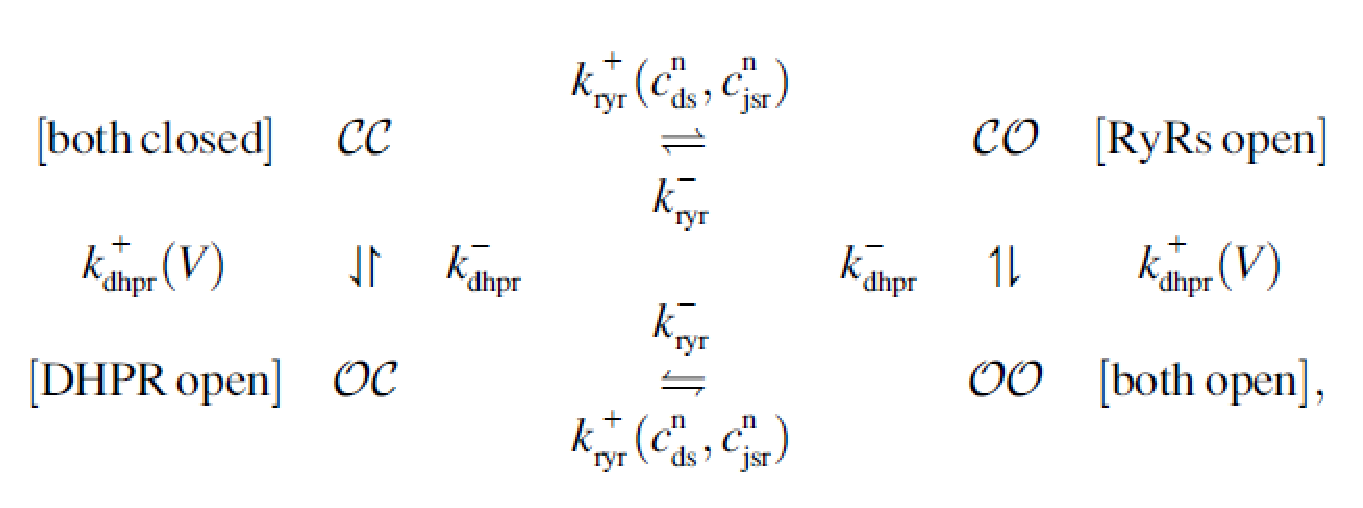
\includegraphics[height=3.5cm,
    angle=0]{./images/Blair_CRU.eps}}
\caption{4-state CRU minimal model}
\label{fig:Blair_CRU}
\end{figure}


{\bf Target}: Model the triggering of CICR during the whole-cell
voltage clamp protocols.


% \subsubsection{ Minimal model for a single RyR channel}
% \label{sec:minimal-model-single}

% In this paper, for the purpose of validating the probability density
% approach which is being introduced in the next section, the Markov
% model of reduced complexity is used, i.e. minimal whole cell
% model\footnote{ minimal model = the most basic model} with each
% channel has 2 states.


% \begin{equation}
%   \label{eq:161}
%   C \ce{<=>[k^+_\ryr(c^n_\ds,c^n_\jsr)][k^-_\ryr]} O  
% \end{equation}
% with the activation {\it rate constant} is calcium ($c_\ds$ and
% $c_\jsr$) dependent, and the inactivation $k^-_\ryr$ is assumed to
% be a constant.

% \subsubsection{Minimal model for a single L-type $\Ca$-channels}
% \label{sec:minimal-model-single-1}

% Assumption: \textcolor{red}{it ignores the $V_m$ and $[\ca]_{ds}$
%   inactivation dependent of DHPR}. However, the paper focuses on
% $V_m$-clamp at which such inactivation can be neglected. 

% \begin{equation}
%   \label{eq:162}
%   C \ce{<=>[k^+_{dhpr}(V)][k^-_{dhpr}]} O    
% \end{equation}
% with the activation is voltage-dependent and the inactivation
% $k^-_\ryr$ is assumed to be a constant.


\subsubsection{Model a CRU}
\label{sec:model-cru}

With one megachannel RyR and one DHPR,
\textcolor{red}{each CaRU is modelled as a 4-state release site} ($M =
4$).
\begin{equation}
  \label{eq:163}
  \begin{array}{c}
    CC \ce{<=>[k^+_\ryr(c^n_{ds},c^n_\jsr)][k^-_\ryr]} CO \\
    k^+_{dhpr}(V) \Updownarrow  k^-_{dhpr}   
    \text{\hspace{10 mm}     } k^-_{dhpr} \Updownarrow  k^+_{dhpr}(V)  \\
    OC \ce{<=>[k^-_\ryr][k^+_\ryr(c^n_{ds},c^n_\jsr)]}OO\\
  \end{array}
\end{equation}

There are totally 2+2N equations, Sect.~\ref{sec:ode-1}: 
\begin{itemize}
\item one for the bulk myoplasm $c_\myo$
\item one for the network SR $c_\nsr$
\item $N$ for the junctional SR $c_\jsr$
\item $N$ for the subspace $c_\ds$
\end{itemize}


\subsection{Mathematical model}
\label{sec:mathematical-model-16}

% \subsubsection{Values for inactivation rates}
% \label{sec:valu-inact-rates}

% Both $k^-_{dhpr}$ and $k^-_\ryr$ are chosen as fixed values so that
% the mean open-time is 0.2ms and maximum open probability for the
% megachannel is 0.1
% \begin{equation}
%   \label{eq:167}
%   \begin{split}
%     k^-_{dhpr} &= constant \\
%     k^-_\ryr &= constant \\      
%   \end{split}
% \end{equation}

% \subsubsection{Values for activation rates}
% \label{sec:valu-activ-rates}

% The rate constant for the activation of the cluster of RyR is a
% sigmoidal function of the dyadic subspace
% [\ce{Ca^2+}]\citep{sobie2002tcas}. As a heterometric protein, RyR is
% assumed to have 4 $\Ca$-binding sites
% \begin{equation}
%   \label{eq:164}
%   k^+_\ryr = \overline{k^+_\ryr} \frac{(c^n_{ds})^4}{(K_\ryr)^4 + (c^n_{ds})^4}
% \end{equation}
% with $\overline{k^+_\ryr}$ is the maximum value, $K_\ryr$ is
% {\bf half-maximal activation} of RyR megachannel, a decreasing
% function of $c^n_\jsr$.
% \begin{equation}
%   \label{eq:166}
%   K_\ryr = K^{max}_\ryr - \alpha_\ryr c^n_\jsr
% \end{equation}

% The rate constant for the activation of the L-type \ce{Ca^2}-channels
% is assumed $V_m$-dependent only~\citep{luo1994dmc_b}.
% \begin{equation}
%   \label{eq:165}
%   k^+_{dhpr} = \overline{k^+_{dhpr}} \frac{e^{(V_m -
%       V^\theta_{dhpr})/\sigma_{dhpr}}}{1+e^{(V_m -
%       V^\theta_{dhpr})/\sigma_{dhpr}} }
% \end{equation}
% with $ \overline{k^+_{dhpr}}$ is the maximum value, $V_m$ is the
% membrane potential, $V^\theta_{dhpr}$ is the reversible potential.


% \subsection{Probability approach for a single type of channel}
% \label{sec:prob-appr-single}

% At first, we examine a single channel.  In general, the activation
% rate for a single a single \ce{Ca^2+} channel can be either
% calcium-dependent, voltage-dependent or both.  For simplicity, we
% first examine the diagram for state transition of a two-state single
% \ce{Ca^2+} channel with the transition rate (in this case it is also
% activation rate) is calcium-dependent,
% \begin{equation}
%   \label{eq:177}
%   C \ce{<=>[k^+c^\eta][k^-]} O
% \end{equation}
% with $[\text{transition rate}]=$T$^{-1}$ (unit of reciprocal
% time). $c$ is the local [\ce{Ca^2+}]\footnote{the concentration of
%   calcium near the \ce{Ca^2+}-regulated site}. 
% \begin{itemize}
% \item $k^+$ is the association rate constant with unit
%   (concentration$^{-\eta}$ .T$^{-1}$). 
% \item $\eta$ is the cooperativity of calcium binding, i.e. denoting
%   the number of binding calcium ions required to activate the channel.
% \end{itemize}

% The state transition above is a discrete-state continuous time
% stochastic process that takes on values in the state space
% $\mathcal{S} = (C,O)$
% (\textcolor{red}{NOTE: the order is important here, as we will use the
%   index to denote the state in the programming code},
% e.g. 1 for C and 2 for O).  $S(t)$ is used to denote the state of the
% channel at the time point $t$.  As the gating is a stochastic process,
% $S(t)$ is a random variable . 

% If we examine more than one channel, the state spaces would be of
% higher dimension, e.g. for three channels
% \begin{eqnarray*}
%   \mathcal{S}=\{CCC, CCO, COO, COC ... \},
% \end{eqnarray*}
% yet still a discrete-state continuous time stochastic
% process\citep{mazzag2005erca}. Normally, we're only interested in the
% number of channels in a particular states. Thus, to make the problem
% easier to handle, we define a column-vector whose index referring to a
% particular state (that's why we mentioned previously that the order of
% the state in the state space is important) and the values of the
% corresponding index is the number of channels in that state. 

% Example: for a single channel with two states, we have
% $\mathbf{u}_0=[0,1]^T$ or $\mathbf{u}_0=[1,0]^T$. In the more
% complicated situation, i.e. more than two states or more than one
% channels, a combinatoric arrangements should be identified. For
% example, for 3 states and 2 channels
% \begin{verbatim}
% st1 st2 st3
%  2   0   0
%  1   1   0
%  1   0   1
%  0   2   0
%  0   1   1
%  0   0   2
% \end{verbatim}

% % If we examine more than one type of channel, the state spaces would be
% % of higher dimension, e.g. for two types of channels
% % \begin{eqnarray*}
% %   \mathcal{S}=\{C_1C_2, C_1O_2, O_1O_2, O_1C_2\},
% % \end{eqnarray*}
% % yet still a discrete-state continuous time stochastic
% % process\citep{mazzag2005erca}. If we examine a CaRU, this state space
% % will be explosive as we may have a bunch of channels for each
% % type. Thus,
% % \textcolor{red}{we will learn using algebraic representation (matrix,
% %   vector) to represent the states}.

% \subsubsection{Algebraic representation}
% \label{sec:algebr-repr}

% All rate transitions in the state space for the dichotomous situation
% above can be represented using the idea of the famous
% {\bf telegraph process} is
% used\footnote{\url{http://en.wikipedia.org/wiki/Telegraph_process}}.
% This is a memoryless continuous-time stochastic process,
% % At a given time instance, the local [\ce{Ca^2+}] is constant,
% % e.g. equal to the fixed background [\ce{Ca^2+}] denoted by $c_\infty$,
% then the {\it Q-matrix} (the infinitesimal matrix) of that process is
% \begin{equation}
%   \label{eq:179}
%   Q = (q_{ij}) = \left( 
%     \begin{array}{cc}
%       -k^+c^\eta & k^+c^\eta\\
%       k^- & -k^-\\
%     \end{array}
%   \right)
% \end{equation}
% The off-diagonal elements $q_{ij}$ ($i\ne j$) of the infinitesimal
% generator matrix (Q-matrix) is itself the transition rate (i.e. the
% probability) from state $i$-th to state $j$-th per unit time.
% \begin{equation}
%   \label{eq:181}
%   q_{ij} = \lim_{\Delta \rightarrow 0} \frac{Prob[S(t+\Delta t) = \mathcal{S}_j| S(t)
%     =\mathcal{S}_i ]}{\Delta t}
% \end{equation}

% For easier manipulation in programming, this Q-matrix can be
% decomposed into two separate matrices $K_-$ and $K_+$ (or some others
% use $K_m$ and $K_p$ with $m=minus, p=plus$).
% \begin{equation}
%   \label{eq:180}
%   Q =  \left( 
%     \begin{array}{cc}
%       0 & 0\\
%       k^- & -k^-\\
%     \end{array}
%   \right) + c^\eta  \left( 
%     \begin{array}{cc}
%       -k^+ & k^+\\
%       0 & 0\\
%     \end{array}
%   \right)
% \end{equation}
% with
% \begin{equation}
%   \label{eq:388}
%   K_m =  \left( 
%     \begin{array}{cc}
%       0 & 0\\
%       k^- & -k^-\\
%     \end{array}
%   \right); \; K_p =  \left( 
%     \begin{array}{cc}
%       -k^+ & k^+\\
%       0 & 0\\
%     \end{array}
%   \right)  
% \end{equation}

% Now, we examine the \ce{Ca^2+}-inactivation process.
% \begin{equation}
%   \label{eq:193}
%   O \ce{<=>[k^+c^\eta][k^-]} C
% \end{equation}
% In this situation, the Q-matrix would be the same if we invert the
% order of the states, i.e. (1,2) = (O,C)=$\mathcal{S}$.

% % To make the problem easier to handle, we define a column-vector whose
% % elements are 1 if the channel is open, and 0 otherwise. Thus, for the
% % \ce{Ca^2+}-activated process, $\mathbf{u}_0=[0,1]^T$; while for the
% % \ce{Ca^2+}-inactivated process, $\mathbf{u}_0=[1,0]^T$. In the more
% % complicated situation, e.g. more than two states, a combinatoric
% % arrangements should be identified, e.g. for 3 states and 3 channels


% % \begin{verbatim}
% % 2 0 0 

% % \end{verbatim}

% However, due to the effect of the residual \ce{Ca^2+} on
% channels~\citep{mazzag2005erca}, the local [\ce{Ca^2+}] will generally
% not be given the constant values, but rather decrease or increase
% depending on the channels are closed or open. Thus, although the
% stochastic process given by $S(t)$, and $c(t)$ has the Markov
% property, the Markov chain $S(t)$ is {\it time-inhomogeneous} as the
% transition rate is not constant but rather functions of time.

% \subsection{Probability approach for CaRU model - bivariate}
% \label{sec:prob-appr-caru-1}

% In the previous section, we described the probability approach of a
% single type of ion channel. As single CaRU has two types of ion
% channels, there is an important difference we need to discriminate:
% the state of a single channel and the state of a release site. Thus,
% in general, we need two vectors $U_R, U_L$, whose elements are vectors
% of denoting the state of the release site, i.e. $u_{R,i}$ is the
% vector whose elements $u_{R,i}[j]$ denoting the number of L-type
% channels in the state $j$ of L-type, $v_{R,i}$ is the vector whose
% elements $u_{L,i}[j]$ denoting the number of RyR channels in the state
% $j$ of RyR.

% When the number of CaRU is large, then the selection of a single CaRU
% can be considered as a random process. The state space $\mathcal{S}$
% of a release site, as described in the previous section, is dependent
% on the number of states of a single type of channel, and the number of
% channels for each type. For validation of the method, i.e. the
% probability approach, the minimum whole cell model and the all-or-none
% behavior of RyR megachannel, as well as DHPR channel, was
% assumed. Under that assumption, the state space of one CaRU is
% $\mathcal{S} = \{CC, CO, OO, OC\}$ with 4 elements. The first index of
% a state is the state of DHPR, the second index of a state is the state
% of RyR.

% If there is a large number of CaRUs, then at any time $t$, one could
% randomly sample one CaRU from the population to produce an instance of
% the random variables $\tilde{S}(t)$. To make it complete, we need to
% define a measure on $\tilde{S}(t)$, i.e. the probability
% distribution. Based on the model described in the previous section, a
% state of a CaRU is determined by two concentrations ($c^n_\jsr,
% c^n_{ds}$) with $n$ is a randomly selected index. As the
% concentrations, denoted by $\tilde{c}_{ds}(t), \tilde{c}_\jsr(t)$ are
% continuous random variables, their instances are denoted by
% $[c_{ds},c_{ds}+dc_{ds}],[c_\jsr, c_\jsr+dc_\jsr]$, respectively.

% As a result, the gating mechanism can be represented using a
% probability density function conditioned on its state. This is a
% continuous multivariate probability density functions of both the
% \ce{Ca^2+} concentrations in dyadic subspace ($\tilde{c}_{ds}(t)$) and
% junctional SR ($ \tilde{c}_\jsr(t)$) given its state, at time $t$, is $i$.
% % Finally, the probability to select a CaRU and its the state is $i$ at a time
% % point $t$ is the
% % for 
% % , that
% % is
% % \begin{multline}
% %   \label{eq:195}
% %   \rho^i(c_{ds},c_\jsr,t) dc_{ds}dc_\jsr =&
% %   Prob((c_{ds}<\tilde{c}_{ds}(t) < c_{ds} + dc_{ds}) \cap \\
% %   &(c_\jsr<\tilde{c}_\jsr(t) < c_\jsr + dc_\jsr) \cap \\
% %   &\tilde{S}(t)=i )
% % \end{multline}

% \begin{eqnarray*}
%   \rho^i(c_{ds},c_\jsr,t) dc_{ds}dc_\jsr =&
%   Prob((c_{ds}<\tilde{c}_{ds}(t) < c_{ds} + dc_{ds}) \cap \\
%   &(c_\jsr<\tilde{c}_\jsr(t) < c_\jsr + dc_\jsr) \cap \\
%   &\tilde{S}(t)=i )
% \end{eqnarray*}

% {\bf TIPS}: The index for the state of a CaRU is denoted by $i$ ($1\le
% i \le M$), while $n$ is the index for a CaRU ($1 \le n \le N$). In the
% probability density approach, $N$ is no longer used.

% There are totally $M=4$ probability density functions to examine.
% Now, we study the dynamics, i.e. the change, in these
% density functions. The change in probability at a particular states are
% due to (1) the change in state ($i$ to $j$) (reaction), (2) the change in
% concentration $c_{ds}, c_\jsr$ (advection diffusion).

% Let's break down the situation.
% \begin{itemize}
% \item If the current state is CC (the first C is the state of DHPR and
%   the second C is the state of RyR), then the next possible state is
%   CO or OC. Given that
%   \begin{equation}
%     \label{eq:194}
%     \begin{split}
%       C \ce{<=>[k^+_{dhpr}][k^-_{dhpr}]} O;      C \ce{<=>[k^+_\ryr][k^-_\ryr]} O 
%     \end{split}
%   \end{equation}

%   The probability of state transition for CC, thus, is denoted by
%   \begin{equation}
%     \label{eq:197}
%     k^-_\ryr\rho^{CO} + k^-_{dhpr} \rho^{OC} - (k^+_{dhpr}+k^+_\ryr)\rho^{CC}
%   \end{equation}

% \item If the decrease in concentration is represented by the {\bf advection
%     rate} $f^i_{ds}, f^i_\jsr$. Thus, the downward change in
%   concentration has the negative effect on the probability.  We take
%   the example for the case of CC state
%   \begin{equation}
%     \label{eq:198}
%     -\frac{\partial}{\partial c_{ds}}[f^{CC}_{ds}\rho^{CC}] -\frac{\partial}{\partial c_\jsr}[f^{CC}_\jsr\rho^{CC}]
%   \end{equation}
% \end{itemize}

% For this multivariate probability density to be consistent with the
% dynamics of the Monte Carlo model of cardiac EC coupling, in essence,
% the change in 4 probability density functions are represented by a set
% of four advection-reaction equations (note the first index is DHPR)
% \begin{equation}
%   \label{eq:196}
%   \begin{split}
%     \frac{\partial \rho^{CC}}{\partial t} &=   -\frac{\partial}{\partial  c_{ds}}[f^{CC}_{ds}\rho^{CC}] -\frac{\partial}{\partial
%       c_\jsr}[f^{CC}_\jsr\rho^{CC}] + k^-_\ryr\rho^{CO} + k^-_{dhpr} \rho^{OC} - (k^+_{dhpr}+k^+_\ryr)\rho^{CC} \\ 
%     \frac{\partial \rho^{CO}}{\partial t} &=  -\frac{\partial}{\partial  c_{ds}}[f^{CO}_{ds}\rho^{CO}] -\frac{\partial}{\partial
%       c_\jsr}[f^{CO}_\jsr\rho^{CO}] + k^-_\ryr\rho^{CC} + k^-_{dhpr}
%     \rho^{OO} - (k^+_{dhpr}+k^+_\ryr) \rho^{CO} \\
%     \frac{\partial \rho^{OO}}{\partial t} &= -\frac{\partial}{\partial  c_{ds}}[f^{OO}_{ds}\rho^{OO}] -\frac{\partial}{\partial
%       c_\jsr}[f^{OO}_\jsr\rho^{OO}] + k^-_\ryr\rho^{OC} + k^-_{dhpr}
%     \rho^{CO} - (k^+_{dhpr}+k^+_\ryr) \rho^{OO}   \\
%     \frac{\partial \rho^{OC}}{\partial t} &=  -\frac{\partial}{\partial  c_{ds}}[f^{OC}_{ds}\rho^{OC}] -\frac{\partial}{\partial
%       c_\jsr}[f^{OC}_\jsr\rho^{OC}] + k^-_\ryr\rho^{OO} + k^-_{dhpr}
%     \rho^{CC} - (k^+_{dhpr}+k^+_\ryr) \rho^{OC}  
%   \end{split}
% \end{equation}
% \textcolor{red}{Here we have total 8 unknown parameters,} $f^i_{ds},
% f^i_\jsr$ ($i=\overline{1..4}$).

% Noting that this can be compactly represented using matrix form
% \begin{equation}
%   \label{eq:204}
%   \frac{\partial \rho^i}{\partial t} = - \frac{\partial}{\partial
%     c_{ds}}[f^i_{ds}\rho^i] - \frac{\partial}{\partial
%     c_\jsr}[f^i_\jsr\rho^i]  + [Q\rho]^i
% \end{equation}
% with $[\rho Q]^i$ is the $i$-th element of the vector-matrix
% multiplication $ Q\rho$ (size: $M\times 1$).  The infinitesimal generator matrix (Q-matrix) is
% \begin{equation}
%   \label{eq:211}
%   \begin{array}{ccccc}
%     & CC & CO & OO & OC \\
%     CC  & -(k^+_\ryr+k^+_{dhpr}) & k^+_\ryr  & 0  & k^+_{dhpr} \\
%     CO  &  k^-_\ryr & -(k^-_\ryr +k^+_{dhpr})  & k^+_{dhpr} & 0\\
%     OO   & 0 & k^-_{dhpr} &-(k^-_{dhpr}+k^-_\ryr )  & k^-_\ryr \\
%     OC   & k^-_{dhpr}  & 0 & k^+_\ryr & -(k^-_{dhpr}+k^+_\ryr) \\
%   \end{array}
% \end{equation}
% {\bf TIPS}: Note the special characteristic of this matrix - the sum
% of elements on each row is zero.

% Finally, we use the notation $\rho$ as a column-vector
% \begin{equation}
%   \label{eq:212}
%   \rho = \left[
%     \begin{array}{c}
%       \rho^{CC} \\
%       \rho^{CO} \\
%       \rho^{OO} \\
%       \rho^{OC}
%     \end{array}
%   \right]
% \end{equation}


% {\bf idenfity 8} with the advection rates are functions of $c_{ds},
% c_\jsr$
% \begin{equation}
%   \label{eq:200}
%   \begin{split}
%     f^i_{ds} &= \frac{1}{\lambda^T_{ds}} \left( \gamma^i_{dhpr}J^T_{dhpr}
%       + \gamma^i_\ryrJ^T_\ryr - J^T_{efflux}  \right) \\
%     f^i_\jsr &= \frac{1}{\lambda^T_\jsr} \left(J^T_{refill}
%       - \gamma^i_\ryrJ^T_\ryr  \right) 
%   \end{split}
% \end{equation}
% with $\gamma^T_{ds} = N\gamma_{ds}$, $\gamma^T_\jsr =
% N\gamma_\jsr$. In these 8 equations, we have 4 unknown fluxes.  The
% four fluxes that may influences the dyadic subspace and junctional SR
% are
% \begin{eqnarray*}
%   J^T_\ryr &= v^T_\ryr (c_\jsr - c_{ds})\\
%   J^T_{efflux} &= v^T_{efflux} (c_{ds} - c_{myo}(t)) \\
%   J^T_{refill} &= v^T_{refill} (c_{nsr}(t) - c_\jsr) \\
%   J^T_{dhpr} &= -A_m P^T_{dhpr} \frac{V}{V_\theta} \left( \frac{c^n_{ds}e^{V/V_\theta}-[\Ca]_o}{e^{V/V_\theta}-1}  \right) 
% \end{eqnarray*}
% These equations involve the two dynamics quantities [\ce{Ca^2+}] of bulk myoplasmic ($c_{myo}(t)$) and
% network SR ($c_{nsr}(t)$) are time-variant quantities which satisfy the ODEs
% \begin{eqnarray*}
%   \frac{dc_{myo}}{dt} &= J_{leak} + J^*_{efflux} - J_{NCX} - J_{SERCA}
%   + J_{in} \\
%   \frac{dc_{nsr}}{dt} &= \frac{1}{\lambda_{nsr}} (J_{SERCA} -  J^*_{refill} - J_{leak})
% \end{eqnarray*}
% with $J_{leak}, J_{SERCA}, J_{in}$ are determined using the equations
% in the Monte Carlo approach. The only difference is with the
% $J^*_{efflux}$ and $J^*_{refill}$ which are the function of $c_{ds}$
% and $c_\jsr$. In other words, they are functional form of the
% probability densities
% \begin{eqnarray*}
%   J^*_{efflux} = \int^\infty_0 \int^\infty_0 v^T_{efflux} \left[ c_{ds}
%     - c_{myo}(t)  \right] \rho^T(c_{ds},c_\jsr, t)dc_{ds}dc_\jsr\\
%   J^*_{refill} =  \int^\infty_0 \int^\infty_0 v^T_{refill} \left[ c_{nsr}(t)
%     - c_\jsr  \right] \rho^T(c_{ds},c_\jsr, t)dc_{ds}dc_\jsr
% \end{eqnarray*}
% where $\rho^T(c_{ds},c_\jsr,t) = \sum_{i=1}^M \rho^i$ is the total
% probability distribution of the dyadic subspace and junctional SR
% irrespective of the state of a randomly sampled CaRU.

% The probability density approach produce the distribution of
% [\ce{Ca^2+}] in (1) dyadic subspace and (2) junctional SR based on a
% system of partial differential equations, eq.~\eqref{eq:196}.

\subsubsection{ODEs}
\label{sec:ode-1}

\begin{framed}
  Suppose the concentration of a species is $c$, defined over volume
  $V$. However, in cell, a large part is buffered, suppose the
  buffering factor is $\beta_1$ ($0<\beta_1<1$). So, the free amount
  if $cV\beta_1$, or the concentration defined over $V$ is indeed
  $c\beta_1$. If we still use $c$ as the concentration of the species
  in cell, it should be defined over an effective volume
  $V/\beta_1$. By doing this, we don't have to remap the concentration
  using the buffering factor $dc/dt=\beta\times (\sum J)$, rather we
  will use $ dc/dt = \frac{1}{\lambda}(\sum J)$ with $\lambda$ is the
  volume fraction. 

  This kind of convention is being used in~\citep{williams2007pda}, while
  the use of real volume, and multiple the flux with buffering factor
  $\beta$ is being used in~\citep{williams2011}
  (Sect.~\ref{sec:williams-...-jafri}).
\end{framed}

Based on the above reasoning, all the concentrations should be defined
over their corresponding effective volume, e.g. $V_\ds/\beta_\ds$,
$V_\myo/\beta_\myo$,...  As all fluxes are defined over $V/\beta_1$,
so to map to the corresponding effective volume, say $\hat{V}_\ds
=V_\ds/beta_\ds$, we need to multiply
$\frac{\hat{V}_\myo}{\hat{V}_\ds}$. 

\textcolor{red}{All the fluxes are defined over myoplasmic effective
  volume $\hat{V}_\myo=\frac{V_\myo}{\beta_\myo}$}.
Yet the concentrations are defined based on the effective volume of
the corresponding compartment, so we need to multiple $\hat{V}_\myo$
and then divided by the effective volume of that compartment, which is
formulated via the effective volume ratio $\lambda$.
\begin{eqnarray}
  \label{eq:1006}
  \frac{dc_{myo}}{dt} &&=  J_{leak}+J^T_{efflux} - J_{NCX} - J_{SERCA} +
  J_\bCa \\
  \frac{dc_{nsr}}{dt} &&= \frac{1}{\lambda_{nsr}} \left( -J_{leak} +
    J_{SERCA} - J^T_{refill} \right)\\
  \frac{dc^n_\jsr}{dt} &&= \frac{1}{\lambda_\jsr} \left( J^n_{refill} -J^n_{ryr} \right)\\
  \frac{dc^n_{ds}}{dt} &&= \frac{1}{\lambda_{ds}} \left( J^n_{ryr} -J^n_{efflux} \right)
\end{eqnarray}
with $1\le n\le N$. The total contribution of efflux from all
subspaces to bulk myoplasm, and from network SR to all junctional SR
are
\begin{eqnarray}
  \label{eq:1007}
  J^T_\ef &&= \sum^N_{n=1} J^n_\ef \\
  J^T_\rf &&= \sum^N_{n=1} J^n_\rf \\
\end{eqnarray}
The effective volume ratios $\lambda_\nsr,\lambda_\jsr,\lambda_\ds$.
\begin{eqnarray}
  \label{eq:1010}
  \lambda_\nsr &&= \frac{\hat{V}_\nsr}{\hat{V}_\myo}= \frac{V_\nsr/\beta_\nsr}{V_\myo/\beta_\myo} \\
  \lambda_\jsr &&= \frac{V_\jsr/\beta_\jsr}{V_\myo/\beta_\myo} =
  \frac{1}{N} \frac{V^T_\jsr/\beta_\jsr}{V_\myo/\beta_\myo}  \\
  \lambda_\ds &&= \frac{V_\ds/\beta_\ds}{V_\myo/\beta_\myo} =\frac{1}{N}\frac{V^T_\ds/\beta_\ds}{V_\myo/\beta_\myo} 
\end{eqnarray}

\subsubsection{Fluxes}
\label{sec:fluxes-4}

All the fluxes are defined over $\hat{V}_\myo$, i.e. all the transfer
rates [1/sec] and permeability are mapped to this volumes.
\begin{enumerate}
\item The influx of $\Ca$ through DHPR $J^n_\dhpr$ in the subspace,
  yet defined over myoplasmic volume, is
  \begin{equation}
    \label{eq:1015}
    J^n_\dhpr = -\frac{\Csc A_{cap}}{z_\ca F \hat{V}_\myo}I^n_\dhpr
  \end{equation}
  where specific membrane capacitance $\Csc = 1\mu$F/cm$^2$, $A_{cap}$
  is the capacitive area of the membrane [cm$^2$], and the effective
  myoplasmic volume $\hat{V}_\myo = \frac{V_\myo}{\beta_\myo}$ (pL), and
  the inward current $I^n_\dhpr<0$ is
  \begin{equation}
    \label{eq:1016}
    I^n_\dhpr = \gamma^n_\dhpr \frac{P^T_\dhpr}{N}\left(\frac{z_\ca
        FV_m}{V_\theta}\right) \left( \frac{c^n_\ds
        e^{V_m/V_\theta}-[\Ca]_o}{e^{V_m/V_\theta}-1}\right)  \;\;\text{[pA/$\mu$F]}
  \end{equation}
  where $V_\theta = \frac{RT}{z_\ca F}$, $P^T_\dhpr$ is the total
  (whole-cell) permeability of the DHPR [cm/s], $\gamma^n_\dhpr$ is the
  random variable that is 0 or 1 when the DHPR associated with the
  $n$-th CRU is closed, or open, respectively (see ref. in JRW model,
  eq.~\eqref{eq:779}).
  \textcolor{red}{The value of $\gamma$ define the stochastic behavior
    of the model}.

\item The release flux $J^n_\ryr$ is assumed follow Fickian's diffusion
  \begin{equation}
    \label{eq:1017}
    J^n_\ryr = \gamma^n_\ryr \frac{v^T_\ryr}{N}\left( c^n_\jsr-c^n_\ds\right)
  \end{equation}
  where $\gamma^n_\ryr$ is the random variable that is 0 or 1 when the
  RyR2 associated with the $n$-th CRU is closed, or open, respectively.


\item 
  The diffusion from each subspace to the bulk myoplasm is
  \begin{equation}
    \label{eq:1018}
    J^n_\ef =  \frac{v^T_\ef}{N}\left( c^n_\ds-c_\myo \right)
  \end{equation}


\item The diffusion from network SR to each subspace is
  \begin{equation}
    \label{eq:1019}
    J^n_\rf =  \frac{v^T_\rf}{N}\left( c_\nsr-c^n_\jsr \right)
  \end{equation}


\item The background $\Ca$ influx $I_\bCa$ (or $J_{in}$ in the paper)
  is~\citep{rice1999mgg}
  \begin{equation}
    \label{eq:1020}
    J_\bCa = -\frac{\Csc A_{cap}}{z_\ca F \hat{V}_\myo}I_\bCa
  \end{equation}
  with 
  \begin{eqnarray}
    \label{eq:1026}
    I_\bCa&&=g_\bCa(V_m-E_\ca) \\
    E_\ca &&= \frac{RT}{z_\ca F}\ln\frac{c_o}{c_\myo}
  \end{eqnarray}


\item The flux of $\Ca$ via Na/Ca exchanger $J_\ncx$ is
  \begin{equation}
    \label{eq:1021}
    J_\ncx = -\frac{\Csc A_{cap}}{z_\ca F\hat{V}_\myo}I_\ncx
  \end{equation}
  where ~\citep{luo1994dmc_a,jafri1998cad,rice1999mst}
  \begin{equation}
    \label{eq:1024}
    \begin{split}
      I_\ncx = \overline{I}_\ncx \frac{1}{\left(K^3_{m,NCX.Na}+[\ce{Na}]_0^3\right)
        \left(K_{m,Ca}+[\ce{Ca}]_o\right)\left(1+k^{sat}_{NCX}\exp[(\eta_\ncx-1).\frac{V_m}{RT/F}]\right)}
      \\
      \times\left(\exp[\eta_\ncx\frac{V_m}{RT/F}] [\ce{Na}]_i^3 [\ce{Ca}]_o -
        \exp[(\eta_\ncx-1)\frac{V_m}{RT/F}] [\ce{Na}]_o^3 [\ce{Ca}]_i\right)
    \end{split}
  \end{equation}
  with
  \begin{itemize}
  \item 3Na:1Ca ratio

  \item $K_{m,NCX.Na}=87.5\times 10^3\mu$M, $K_{m,NCX.Ca}=1.38\times
    10^3\mu$M are $\Na$ and $\Ca$ half-saturation constant,
    respectively.

  \item $\overline{I}_\ncx=150\mu A.\mu F^{-1}$ (previously $k_{Na/Ca}$): the
    maximum of Na/Ca current.

  \item $k^{sat}_{NCX}=0.1$ saturation factor to ensure saturation at
    very negative potential

  \item $\eta_\ncx = 0.35$: the position of the energy barrier that
    control $V_m$-dependent (vary between 0 and 1)
  \end{itemize}


\item The SERCA pump $J_\serca$ use~\citep{shannon2000rms}
  (Sect.~\ref{sec:shannon-et-al})
  \begin{equation}
    \label{eq:1022}
    J_\serca = v_\serca
    \frac{\left(\frac{c_\myo}{K_{m.f}}\right)^{\eta_{f.s}}-
      \left(\frac{c_\myo}{K_{m.f}}\right)^{\eta_{f.s}}}{1+\left(\frac{c_\myo}{K_{m.f}}\right)^{\eta_{f.s}}+
      \left(\frac{c_\myo}{K_{m.f}}\right)^{\eta_{f.s}}}
  \end{equation}
  with 
  \begin{itemize}
  \item the maximum rate in either direction are the same, and equal to
    $v_\serca=8.6\mu$M/s. 

  \item the Hill-parameter for the serca in forward (f.s) and reverse
    (r.s) mode is $\eta_{f.s},\eta_{r.s}$, respectively (originally
    denoted by $H_f, H_r$).

  \item the forward and reverse half-saturation (dissociation) constants
    for the SERCA pump are $K_{m.f}=0.17\mu$M, $K_{m.r}=1702\mu$M
  \end{itemize}


\item The passive leak in network SR $J_\leak$ is
  \begin{equation}
    \label{eq:1023}
    J_\leak = g_\leak(c_\nsr-c_\myo)
  \end{equation}
\end{enumerate}


\subsection{Data analysis}
\label{sec:data-analysis-4}

Overall myoplasmic $[\ca]$ involves bulk myoplasm and each of the N
dyadic subspaces (scaled by the effective volumes)
\begin{equation}
  \label{eq:1013}
  \begin{split}
    \hat{c}_{\myo\&\ds} &= \frac{\hat{V}_\myo c_\myo+\hat{V}_\ds
      \sum^N_{n=1} c^n_\ds}{\hat{V}_\myo+N \hat{V}_\ds} \\
    &= \frac{\hat{V_\myo} c_\myo+\hat{V}^T_\ds
      c^{avg}_\ds}{\hat{V}_\myo+\hat{V}^T_\ds} 
  \end{split}
\end{equation}
with the average dyadic subspace
$c^{avg}_\ds=\frac{1}{N}\sum^N_{n=1}c^n_\ds$. 

Overall SR $[\ca]$ involves the network SR and each of the N
junctional SR (scaled by the effective volumes)
\begin{equation}
  \label{eq:1014}
  \begin{split}
    \hat{c}_{\nsr\&\jsr} &= \frac{\hat{V}_\nsr c_\nsr+\hat{V}_\jsr
      \sum^N_{n=1} c^n_\jsr}{\hat{V}_\nsr+N \hat{V}_\jsr} \\
    &= \frac{\hat{V_\nsr} c_\nsr+\hat{V}^T_\jsr
      c^{avg}_\jsr}{\hat{V}_\nsr+\hat{V}^T_\jsr} 
  \end{split}  
\end{equation}
with the average junction SR $c^{avg}_\jsr=\frac{1}{N}\sum^N_{n=1}c^n_\jsr$.

\begin{framed}
  
  \begin{equation}
    \label{eq:1011}
    \begin{split}
      \frac{dc}{dt} &= V_\myo \frac{dc_\myo}{dt} + V_\nsr
      \frac{dc_\nsr}{dt} + \sum^N_{n=1} V_\jsr \frac{dc_\jsr}{dt} +
      \sum^N_{n=1} V_\ds \frac{dc_\ds}{dt} \\
      &= V_\myo \frac{dc_\myo}{dt} + V_\nsr
      \frac{dc_\nsr}{dt} + NV_\jsr \frac{1}{N}\sum^N_{n=1} \frac{dc_\jsr}{dt} +
      NV_\ds \frac{1}{N}\sum^N_{n=1} \frac{dc_\ds}{dt} \\
      &= V_\myo \frac{dc_\myo}{dt} + V_\nsr
      \frac{dc_\nsr}{dt} + V^T_\jsr \frac{1}{N}\sum^N_{n=1} \frac{dc_\jsr}{dt} +
      V^T_\ds \frac{1}{N}\sum^N_{n=1} \frac{dc_\ds}{dt} 
    \end{split}
  \end{equation}
  Based on the conservation of calcium in a closed cell, then
  $\frac{dc}{dt}=0$, then 
  \begin{equation}
    \label{eq:1012}
    \frac{dc_\myo}{dt} + \frac{V_\nsr}{V_\myo}
    \frac{dc_\nsr}{dt} + \frac{V^T_\jsr}{V_\myo} \frac{1}{N}\sum^N_{n=1} \frac{dc_\jsr}{dt} +
    \frac{V^T_\ds}{V_\myo} \frac{1}{N}\sum^N_{n=1} \frac{dc_\ds}{dt} = 0 
  \end{equation}
  and the sum of all the fluxes equal to 0. 
\end{framed}

\subsection{Validate the model}
\label{sec:validate-model}

To validate the novel probability density approach, traditional Monte
Carlo simulation of graded, locally controlled SR \ce{Ca^2+} release
is utilized.

\subsubsection{MC simulations}
\label{sec:mc-simulations}

Solving $2+2N$ ODEs, applying the holding potential of $-80$mV
followed by 20ms duration of test potential $-30, -20, -10$ mV. The
\ce{Ca^2+} release exhibited by this MC model is graded with changes
in membrane potential and depolarization duration, the phenomena that
are not observed in the common-pool model of EC coupling.


In MC approach, $2N+2$ ODEs are solved to determine the dynamics of
[\ce{Ca^2+}] in the dyadic subspace and junctional SR associated with
$N$ CaRUs. In probability density approach, the time-dependent
bivariate probabilities are updated using 4 ODEs. The number of ODEs
in the later approach is equal to the number of states of a CaRU.


..............

\subsection{Analysis the dynamics of a CaRU}
\label{sec:analys-dynam-caru}

In the previous probability density approach, 4 ODEs of
advection-reaction equations are solved numerically. As shown in
Fig.~\ref{fig:Ca_ds_jsr}, when the DHPR initially open ($CC-->OC$), an
influx of trigger \ce{Ca^2+} leads to $\approx 7\mu$M in $c_{ds}$ and
causes the RyR cluster to open ($OC-->OO$). The resulting CICR
mechanism quickly drives the $c_{ds}$ to $\approx 150\mu$M. Note that
the junctional SR depletion is nearly complete ($c_\jsr\approx 0$)
before the $CO-->CC$ transition to complete the CICR cycle. 

\begin{figure}[hbt]
  \centerline{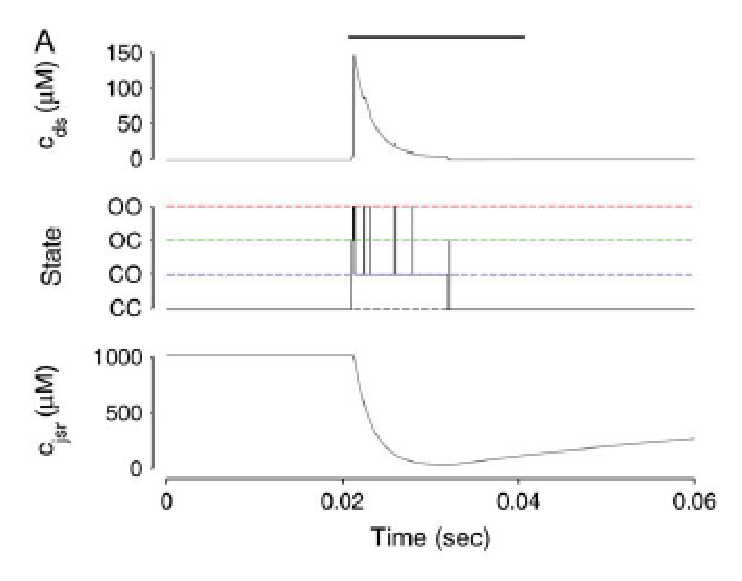
\includegraphics[height=5cm]{./images/Ca_ds_jsr.eps}}
  \caption{The dynamics of [\ce{Ca^2+}] in dyadic subspace and
    junctional SR}
  \label{fig:Ca_ds_jsr}
\end{figure}

The dynamics of $c^n_{ds}$ is much faster than that of $c^n_\jsr$, as
shown in Fig.~\ref{fig:Ca_ds_jsr}. Thus, based on the model
parameters, $c^n_{ds}$ reach the equilibrium swiftly or
\begin{equation}
  \label{eq:210}
  dc^n_{ds}/dt  = 0
\end{equation}
Substituting this equation to the left side of eq.~\eqref{eq:183}, the
solution is
\begin{equation}
  \label{eq:220}
  \overline{c^n_{ds}} =
  \frac{\gamma^n_{dhpr}J^0_{dhpr}+v^T_{efflux}c_{myo}+\gamma^n_\ryr v^T_\ryr
    c^n_\jsr}{\gamma^n_\ryr v^T_\ryr + v^T_{efflux}
    - \gamma^n_{dhpr}J^1_{dhpr}}
\end{equation}
with $J^0_{dhpr}, J^1_{dhpr}$ are functions of plasma membrane voltage
\begin{equation}
  \label{eq:221}
  \begin{split}
    J^0_{dhpr} = \frac{1}{N} \frac{\Csc
      A_{cap}P^T_{dhpr}V}{\hat{V}_\myo V_\theta} \left( \frac{[\Ca]_o}{e^{V/V_\theta}-1}  \right)\\
    J^1_{dhpr} =  -\frac{1}{N} \frac{\Csc
      A_{cap}P^T_{dhpr}V}{\hat{V}_\myo V_\theta} \left( \frac{e^{V/V_\theta}}{e^{V/V_\theta}-1}  \right)
  \end{split}
\end{equation}
that satisfy
\begin{equation}
  \label{eq:2082}
  J^n_{dhpr} =   \gamma^n_{dhpr} (J^0_{dhpr} + \overline{c^n_{ds}}  J^1_{dhpr})
\end{equation}

The solution is split into 2 components (calcium-independent and
$c_\jsr$-dependent):
\begin{equation}
  \label{eq:2051}
  \overline{c^n_{ds}} =   \overline{c^n_{ds,0}} +  \overline{c^n_{ds,1}}  c_\jsr
\end{equation}
with
\begin{equation}
  \label{eq:2061}
  \begin{split}
    \overline{c^n_{ds,0}} &= \frac{\gamma^n_{dhpr}J^0_{dhpr} +
      v_{efflux}c_{myo}}{\gamma^n_\ryr v_\ryr + v_{efflux} - \gamma^n_{dhpr}J^1_{dhpr}} \\
    \overline{c^n_{ds,1}} &=
    \frac{\gamma^n_\ryr v_\ryr}{\gamma^n_\ryr v_\ryr + v_{efflux}
      - \gamma^n_{dhpr}J^1_{dhpr}} \\
  \end{split}
\end{equation}


\subsection{Probability approach for CaRU model - univariate}
\label{sec:prob-appr-caru}

Based on the previous analysis, it is inferred that at a given state
$i$, the concentration of \ce{Ca^2+} at the dyadic subspace will be at
equilibrium. In other words, $c_{ds}$ at state $i$ is
$\overline{c}^i_{ds}$. 
\begin{equation}
  \label{eq:223}
  \overline{c^i_{ds}} =
  \frac{\gamma^i_{dhpr}J^0_{dhpr}+v^T_{efflux}c_{myo}+\gamma^i_\ryr v^T_\ryr
    c_{jsr}}{\gamma^i_\ryr v^T_\ryr + v^T_{efflux}
    - \gamma^i_{dhpr}J^1_{dhpr}}
\end{equation}
is the function of $c_{myo}(t), c_{jsr}$ and CaRU state $i$.

Correspondingly, the bivariate probability density function can be
well approximated by a univariate probability density function
\begin{equation}
  \label{eq:222}
  \rho^i(c_{ds},c_{jsr},t) = \rho^i(c_{jsr},t)\delta(c_{ds}-\overline{c^i_{ds}})
\end{equation}
with $\delta$ is the unit delta function and
\begin{equation}
  \label{eq:224}
  \rho^i(c_{jsr},t) dc_{jsr} =  Prob \left((c_{jsr}<\tilde{c}_{jsr}(t) <
    c_{jsr} + dc_{jsr}) \text{ and } \tilde{S}(t)=i \right)
\end{equation}
Finally, the resulting advection-reaction equations are
\begin{equation}
  \label{eq:225}
  \begin{split}
    \frac{\partial \rho^{CC}}{\partial t} &=   -\frac{\partial}{\partial
      c_{jsr}}[\overline{f}^{CC}_{jsr}\rho^{CC}] + k^-_\ryr\rho^{CO} + k^-_{dhpr} \rho^{OC} - (k^+_{dhpr}+k^+_\ryr)\rho^{CC} \\ 
    \frac{\partial \rho^{CO}}{\partial t} &=  -\frac{\partial}{\partial
      c_{jsr}}[\overline{f}^{CO}_{jsr}\rho^{CO}] + k^-_\ryr\rho^{CC} + k^-_{dhpr}
    \rho^{OO} - (k^+_{dhpr}+k^+_\ryr) \rho^{CO} \\
    \frac{\partial \rho^{OO}}{\partial t} &= -\frac{\partial}{\partial
      c_{jsr}}[\overline{f}^{OO}_{jsr}\rho^{OO}] + k^-_\ryr\rho^{OC} + k^-_{dhpr}
    \rho^{CO} - (k^+_{dhpr}+k^+_\ryr) \rho^{OO}   \\
    \frac{\partial \rho^{OC}}{\partial t} &=  -\frac{\partial}{\partial
      c_{jsr}}[\overline{f}^{OC}_{jsr}\rho^{OC}] + k^-_\ryr\rho^{OO} + k^-_{dhpr}
    \rho^{CC} - (k^+_{dhpr}+k^+_\ryr) \rho^{OC}  
  \end{split}
\end{equation}

\textcolor{red}{Here, we have only 4 unknown parameters} 
$\overline{f}^i$ ($i=\overline{1..4}$), and $\rho^i= \rho^i_{jsr}$, and

\begin{equation}
  \label{eq:226}
  \begin{split}
    \overline{f^i_{jsr}} &= \frac{1}{\lambda^T_{jsr}}
    (J^T_{refill}-\gamma^i_\ryr J^T_\ryr) \\
    &=  \frac{1}{\lambda^T_{jsr}}
    (v^T_{refill} (c_{nsr}(t)-c_{jsr})-\gamma^i_\ryr v^T_\ryr(c_{jsr}-\overline{c^i_{ds}}(t)))
  \end{split}
\end{equation}
Here, $c_{myo}$ and $c_{nsr}$ are time-variant quantities and thus we
need to define two ODEs which is similar to those of the previous
section. Other parameters are derived similarly to the previous
approach, except for the two quantities
\begin{equation}
  \label{eq:234}
  \begin{split}
    J^*_{efflux} = \sum_{i=1}^M \int^\infty_0 v^T_{efflux} \left[ \overline{c}^i_{ds}
      - c_{myo}(t)  \right] \rho^T(c_{ds},c_{jsr}, t)dc_{ds}dc_{jsr}\\
    J^*_{refill} = \sum_{i=1}^M \int^\infty_0 v^T_{refill} \left[ c_{nsr}(t)
      - c_{jsr}  \right] \rho^T(c_{ds},c_{jsr}, t)dc_{ds}dc_{jsr}
    \
  \end{split}
\end{equation}

The fraction of CaRU in each state at a given time $t$ is
\begin{equation}
  \label{eq:235}
  \pi^i(t) = Pr{\tilde{S}(t) = i} = \int_0^\infty \rho^i_{jsr}(c_{jsr},t)dc_{jsr}
\end{equation}



\subsection{Need to revise}
\label{sec:need-revise}

To study the dynamics of calcium concentrations, ordinary differential
equations of these quantities are built up. As mentioned in the
previous section, there are 3 global calcium concentrations (whole
cell) and 2 local calcium concentration (for each CaRU). Thus, with
$N$ release sites, there are totally $3+2N$ quantities. 


For simplicity, in some models, the dynamics of the extracellular
calcium concentration $c_{ext}$ is neglected as the change is
small. Finally, there are totally $2+2N$ ODEs.

\begin{equation}
  \label{eq:168}
  \frac{dc_{myo}}{dt} =  J_{leak}+J^T_{efflux} - J_{NCX} - J_{SERCA} +
  J_{in} 
\end{equation}
\begin{equation}
  \label{eq:185}
  \frac{dc_{nsr}}{dt} = \frac{1}{\lambda_{nsr}} \left( -J_{leak} +
    J_{SERCA} - J^T_{refill} \right)
\end{equation}
\begin{equation}
  \label{eq:183}
  \frac{dc^n_{ds}}{dt} = \frac{1}{\lambda_{ds}} \left(  J^n_{ryr} +
    J^n_{HDPR} - J^n_{efflux}  \right), n=\overline{1...N}
\end{equation}
\begin{equation}
  \label{eq:184}
  \frac{dc^n_{jsr}}{dt} = \frac{1}{\lambda_{jsr}} \left( J^n_{refill}
    -J^n_{ryr} \right), n=\overline{1...N}
\end{equation}

For these equations to be determined, all quantities on the right-hand
sides need to be identified. Here, we have totally 13 quantities (10
fluxes and 3 effective volume ratios) to be determined as follows

{\bf identify 3} effective volume ratios: 
\begin{equation}
  \label{eq:186}
  \lambda_{nsr} = \frac{V_{nsr}/\beta_{nsr}}{V_{myo}/\beta_{myo}} 
\end{equation}
\begin{equation}
  \label{eq:187}
  \lambda_{ds} =\frac{V_{ds}/\beta_{ds}}{V_{myo}/\beta_{myo}} = \frac{1}{N}\frac{V^T_{ds}/\beta_{ds}}{V_{myo}/\beta_{myo}}
\end{equation}
\begin{equation}
  \label{eq:188}
  \lambda_{jsr} = \frac{1}{N}\frac{V^T_{jsr}/\beta_{jsr}}{V_{myo}/\beta_{myo}}
\end{equation}
The assumption here is that the individual dyadic subspaces have the
same physical volume, and individual junctional SRs have the same
physical volume, too. 

{\bf TIPS}: There are some new concepts: (1) the physical volume $V$
is the total volume of a compartment, (2) the effective volume is the
maximal volume $\hat{V}$ within which the particles are free to move.
\begin{equation}
  \label{eq:171}
  \hat{V} = \frac{V}{\beta}
\end{equation}
with $\beta$ is the {\it constant-fraction \ce{Ca^2+} buffer capacity}
or buffering factor and is chosen as a constant for each compartment
($\beta_{ds}, \beta_{jsr}, \beta_{nsr}, \beta_{myo}$).

{\bf identify 2}: Next, the first two fluxes are defined
\begin{equation}
  \label{eq:169}
  J^T_{refill} = \sum_{n=1}^N J^n_{refill}
\end{equation}
\begin{equation}
  \label{eq:170}
  J^T_{efflux} = \sum_{n=1}^N J^n_{efflux}
\end{equation}

{\bf identify 4} other fluxes

The diffusion from the $n$-th dyadic subspace to myoplasma is
\begin{equation}
  \label{eq:175}
  J^n_{efflux} =  \frac{v^T_{efflux}}{N} (c^n_{ds} - c_{myo})
\end{equation}
The assumption here is that each individual dyadic subspace have the
same {\it efflux rate} and the total $v^T_{efflux}$ is chosen as
constant.  $N$ is the number of CaRUs and is given.

The diffusion from network SR to the $n$-th junctional SR is
\begin{equation}
  \label{eq:176}
  J^n_{refill} =  \frac{v^T_{refill}}{N} (c_{nsr} - c^n_{jsr})
\end{equation}
The assumption here is that each individual junctional SR receive the
\ce{Ca^2+} fluxes of the same {\it refilling rate} and the total
$v^T_{refill}$ is chosen as constant.  
Both $c_{myo}$ and $c_{nsr}$ are chosen as constant values. 

This is the trigger \ce{Ca^2+} flux
\begin{equation}
  \label{eq:172}
  J^n_{dhpr} = - \frac{A_m}{zF} I^n_{dhpr}
\end{equation}
with 
\begin{equation}
  \label{eq:173}
  \begin{split}
    A_m &= \frac{C_m \beta_{myo}}{V_{myo}}\\
    I^n_{dhpr} &= \gamma^n_{dhpr}\frac{P^T_{dhpr}}{N}\left(
      \frac{zFV}{V_\theta}\right) \left( \frac{c^n_{ds}e^{V/V_\theta}-c_{ext}}{e^{V/V_\theta}-1}  \right)\\
  \end{split}
\end{equation}
\begin{itemize}
\item $\gamma^n_{dhpr}$ is a random variable with binary value: O if
  DHPR channel of the $n$-th CaRU is closed; and 1 otherwise.
\item $P^T_{dhpr}$ is the total (whole-cell) permeability of the DHPR
\item $V_\theta = \frac{RT}{zF}$
\end{itemize}

\begin{equation}
  \label{eq:174}
  J^n_{ryr} = \gamma^n_{ryr} v^n_{ryr} (c^n_{jsr} -
  c^n_{ds}) = \gamma^n_{ryr} \frac{v^T_{ryr}}{N} (c^n_{jsr} - c^n_{ds})
\end{equation}
with $\gamma^n_{ryr} = 0$ (if closed) and 1 (if open),
respectively. The assumption here is that each individual RyR channel
have the same {\it release rate} and the total $v^T_{ryr}$ are chosen as constant.

{\bf identify 4} remaining fluxes

The constant background \ce{Ca^2+} flux is
\begin{equation}
  \label{eq:189}
  J_{in} = -\frac{A_m}{zF}I_{in}
\end{equation}
with $I_{in} = g_{in} (V-V_{\ce{Ca}})$, the reversible potential is
$V_{\ce{Ca}} = \frac{RT}{2F}\ln\frac{c_{ext}}{c_{myo}}$?????? (Nernst equation).

The SERCA-type Ca-ATPase flux is
\begin{equation}
  \label{eq:190}
  J_{SERCA} = v_{SERCA} \frac{\left( \frac{c_{myo}}{K_{fs}}
    \right)^{\eta_{fs}} - \left( \frac{c_{nsr}}{K_{rs}}
    \right)^{\eta_{rs}}} {1 + \left( \frac{c_{myo}}{K_{fs}}
    \right)^{\eta_{fs}} + \left( \frac{c_{nsr}}{K_{rs}} \right)^{\eta_{rs}}}
\end{equation}
with parameters are constants given in Table 3 of the paper.


The leak \ce{Ca^2+} flux is
\begin{equation}
  \label{eq:191}
  J_{leak} = v_{leak} (c_{nsr}-c_{myo})
\end{equation}
with parameters are experimental-chosen constants.

The flux for \ce{Na+}/\ce{Ca^2+} exchange current is
\begin{equation}
  \label{eq:192}
  J_{NCX} = -\frac{A_m}{F}I_{NCX}
\end{equation}
with 
\begin{eqnarray}
  \label{eq:199}
  I_{NCX} = I^0_{NCX} \frac{
    \ce{[Na+]^3_{myo}} c_{ext} e^{\eta_{ncx}\frac{FV}{RT}} - \ce{[Na+]^3_{ext}}c_{myo} e^{\eta_{ncx}\frac{FV}{RT}} 
  }{ 
    \left( K_{ncx,c}+\ce{[Na+]^3_{ext}}  \right) (K_{ncx,c} + c_{ext})
    \left( 1+ k^{sat}_{ncx} e^{(\eta_{ncx}-1)\frac{FV}{RT}}     \right)
  }
\end{eqnarray}
and all parameters are experimental-chosen constants given in Table 1
and 3 of the paper ~\citep{williams2007pda}.

{\bf Assumption}:
\begin{enumerate}
\item External calcium concentration is constant.
\item Individual dyadic subspaces have same physical volume
  $V^n_{ds}=V_{ds}$
\item Individual junctional SRs have same physical volume
  $V^n_{jsr}=V_{jsr}$
\item Individual RyR channels have the same {\it release rate}
  $v^n_{ryr} = v_{ryr}$.
\item Individual dyadic subspace have the same {\it efflux rate}
  $v^n_{efflux} = v_{efflux}$

\end{enumerate}

\section{Mahajan-\ldots-Weiss (2008) - rabbit (alternans)}
\label{sec:mahajan_weiss_2008}

There have been no detailed whole-cell model accurately reproduce dynamics of AP
and $\Ca$ handling at high pacing rates. They all fail to reproduce some key
experiment findings important to cardiac arrhythmogenesis. In particular, under
rapid pacing (such as during intense physical activity or fright), the heart
automatically adjust by shorting both systole and diastole. This allows adequate
contraction and pumping of blood under a wide range of physiological conditions.
However, at fast rate of contraction, not all of the ion channels can recover
from inactivation fully. This results in decreased current, which causes a less
contraction leading to a lack of blood pumping. 

{\bf Restitution} essentialy describe a functional relationship between the
change of AP duration (APD) and the length of quiescent interval (diastolic
interval, DI) preceding it. APD restitution is a form of adaptation to changes
in rate. To show this relation, an {\bf APD restitution curve} is used by
varying DI and plotting the resulting APD at steady-state conditions.
\textcolor{red}{When the slope greater than 1, oscillations called alternans
occur}.

In particular, $\Ca$
transient alternans during rapid pacing with a clamped AP waveform, as observed
in isolated cardiac myocyte \citep{mahajan2008}. 


L-type $\Ca$ channel model is described in Sect.\ref{sec:LCC_Mahajan2008}


\section{Williams-...-Jafri (2011) - $\Ca$ leak}
\label{sec:williams-...-jafri}

SR $\Ca$ content is regulated by
\begin{enumerate}

\item in response to diverse disease (e.g. arrhythmias or Heart
  Failure (HF)), and is

\item phosphorylation by kinases such as PKA or $\Ca$-calmodulin
  dependent kinase II (CaMKiI)~\citep{marx2000,ai2005}.

\item SR $\Ca$ leaks (visible + invisible)

\item SERCA $\Ca$ pumps
\end{enumerate}

The activity, i.e. $P_o$, of RyRs is controlled by different affectors
\begin{enumerate}
\item $[\Ca]_i$ ($[\Ca]_\myo$)

\item lumenal $[\Ca]_\jsr$~\citep{qin2008}

\item phosphorylation state of RyR

\item RyR mutations such as those related to catecholarminergic
  polymorphic ventricular tachycardia (CPVT)

\item allosteric coupled gating~\citep{marx2001}

\item ...
\end{enumerate}
The conditions mentioned above are more severe in 
arrhythmogenic and contribute to $\Ca$ waves, $\Ca$
alternans...~\citep{Wehrens2005}. Thus, it's believed that
understanding $\Ca$ leaks is critical to our understanding ofheart
function during both physiological and pathophysiological conditions. 

\subsection{Hypothesis analysis}
\label{sec:hypothesis-analysis-17}


During systole, RyRs are activated by $\Ca$ influx via in the adjacent
LCC (DHPR) which lead to the local elevations of $\Ca$, known as
evoked $\Ca$ sparks. During diastole, in the absence of LCC $\Ca$
influx, RyRs can still trigger a spark due to its randomness of
opening. These sparks are known as {\bf spontaneous calcium 
  sparks}.
Spontaneous $\Ca$ sparks are rare, with the spark rate 100-150 sparks/cell/sec
that reflects the finite opening rate of the RyR channels~\citep{cheng1993cse}. 

In this paper, the authors introduced a computational model that can
reprouce different forms of $\Ca$ release, especially those invisible by
standard confocal imaging techniques, known as ``invisible'' $\Ca$ leaks. 
\begin{enumerate}
  \item The leak by spontaneous opening of RyR that can trigger a spark
  \item The non-spark events as the result of  the opening of a single or a few
  RyRs (i.e. $\Ca$ quarks) that fail to  trigger a full $\Ca$
  sparks~\citep{brochet2011}.
   \item A third RyR-based $\Ca$ release (also the second form of invisible
leak) is suggested via a small population of non-clustered RyRs termed
``rogue'' RyRs located away from the $\Ca$ release sites
\citep{sobie2006, lukyanenko2007}. These rogue RyRs are thought to
uncouple to each other, and behave independently \citep{xie2010drr}. 
\end{enumerate}

The calcium release via these non-spark pathways is believed to be a significant
leak~\citep{zima2010, santiago2010}, that may contribute to delayed
afterdepolarization (DAD) and consequently arrhythmia in heart failure
(HF)~\citep{shannon2003}.

\begin{framed}
  In this study, the computational model provide an explicit means to
  investigate nano-scale events related $\Ca$ leak not easily measured
  under experimental settings. Five new discoveries:
  \begin{enumerate}
  \item ``invisible'' leaks can be observed, and is quantitatively
    consistent with earlier unexplained experimental findinds

  \item fully stochastic activation and termination of RyRs can be
    accounted for SR $\Ca$ leak, obviating the inclusion of ad-hoc,
    non-RyR mediated $\Ca$ leak flux that is often used by previous
    models (e.g. ~\citep{sobie2002tcas}
    (Sect.~\ref{sec:sobie2002_jafri})). Here, the energetic coupling
    formulation~\citep{groff2008} derived from allosteric behavior
    observed in biological systems~\citep{duke1999}.

  \item SR $\Ca$ levels depend critically on $P_o$ of RyR and vice
    versa 
  \item single RyR openings, while brief, are frequent ($\sim 3000$
    cell$^{-1}$.s$^{-1}$), yet fail to trigger sparks (as the number
    of sparks is about $\sim 130$ cell$^{-1}$.s$^{-1}$), suggesting
    that $\Ca$ spark fidelity in response to single RyR or LCC
    openings are quite low.
  \item \textcolor{red}{Prediction}: The increased RyR activity can
    somewhat paradoxically, lead to increase SR $\Ca$ leak even in the
    presence of decrease SR $\Ca$ content.
  \end{enumerate}
\end{framed}

The model incorporates 20,000 independent release sites (CRUs); each
contains a cluster of RyRs stochastically gating and instantaneously
coupled via $[\Ca]_\ds$ (local subspace). The CRUs are coupled via
bulk $[\Ca]_\myo$.  There is a small fraction (5\%) of diffusely
distributed, non-junctional or ``rogue'' RyRs.

\subsubsection{RyR model}
\label{sec:ryr-model-1}

The RyRs are modeled as 2-state Markov chain. The dynamics of RyRs in
the dyad is modeled using allosteric coupling based
on~\citep{groff2008} (Sect.~\ref{sec:RYR_Groff2008}). In
addition to allosteric coupling, the transition from C to O are
dependent on both $[\Ca]_\ds$ (via Hill coefficient $\eta$) and
$[\Ca]_\sr$ (via luminal regulation function $\phi$),
eq.~\eqref{eq:1121}.

\subsubsection{SERCA $\Ca$ pumps}
%\label{sec:serca-ca-pumps}

SERCA $\Ca$ pumps is based on Tran-Crampin model
(Sect.~\ref{sec:tran-...-crampin}), eq.~\eqref{eq:1128}. This was
chosen as it displays physiological behavior at low $[\Ca]_i$ and is
sensitive to changes in $[\Ca]_\sr$ which is essential, as RyR-based
leak can balance SERCA.

\subsubsection{Na/Ca exchanger}
\label{sec:naca-exchanger}

Na/Ca exchanger is the main pathway for $\Ca$ extrusion from the
myocyte. The formula being used is eq.~\eqref{eq:1161}

\begin{equation}
  \label{eq:1161}
  J_\ncx = \frac{-A_mI_\ncx}{F.V_\myo}
\end{equation}
with
\begin{equation}
  \label{eq:1146}
  I_\ncx=\overline{I}_\ncx\frac{[\Na]_i^3[\Ca]_o\exp(\eta_\ncx\frac{FV}{RT})-}{}
\end{equation}

\subsubsection{Buffering}
\label{sec:buffering-2}

The SR is composed of network SR (NSR) and junctional SR (JSR), each
with appropriate volumes and $\Ca$ buffers. The $\Ca$ buffers are
assumed to be lumped into a single type. 

\textcolor{red}{The effect of mitochondria is ignored in this
  study}~\citep{andrienko2009}. So, no mitochondrial buffering is
taken into account. 


\subsubsection{Transmembrane fluxes}
\label{sec:transmembrane-fluxes}

The plasma membrane has a background $\Ca$ leak
(Sect.\ref{sec:leaky-current}) and two trans-sarcolemmal calcium transporters:
NCX and PMCA to extrude $\Ca$ ions from the cell. 

\begin{framed}
  The cluster of LCC apposing the RyR cluster are disabled for the
  simulation. The main focus now is on diastolic $\Ca$ signaling when
  LCCs are quiescent. 
\end{framed}


\subsection{Mathematical analysis}
\label{sec:math-analys-1}

\begin{enumerate}
\item RyR: 2-state model
  \begin{equation}
    \label{eq:1122}
    \ce{C <=>[\ce{k^+ \times \phi \times ([\ca]_\ds)^{\eta}}][k^-] O}
%    \ce{C <=>[\ce{k^+ $\times \phi \times([\ca]_\ds)^\eta$}][k^-] O}
  \end{equation}
  The luminal gating function is
  \begin{equation}
    \label{eq:1121}
    \phi = \phi_m[\Ca]_\sr + \phi_b
  \end{equation}
  with luminal calcium $[\Ca]_\sr$ will be $[\Ca]_\jsr$ for junctional
  and $[\Ca]_\nsr$ for non-junctional RyRs. 

  If we ignore the arrangement of individual channels, we can use the
  mean-field allosteric coupling approach~\citep{groff2008}
  (Sect.~\ref{sec:allosteric-coupling}) 
  \begin{equation}
    \label{eq:1212}
    \ce{C <=>[k^+\phi\times([\ca]_{\ds})^\eta\chi^'_C][k^-\chi^'_O] O}
%    \ce{C <=>[\text{$k^+\phi\times([\ca]_{\ds})^\eta\chi^'_C$}][k^-\chi^'_O] O}
  \end{equation}

  \begin{equation}
    \label{eq:1126}
    \chi'_C = \exp\left\{-a^*\eta_C\left[N^C_\ryr \mathcal{E}_{C,C} - (N^O_\ryr-1)\mathcal{E}_{O,O}\right]\right\}
  \end{equation}
  and
  \begin{equation}
    \label{eq:1127}
    \chi'_C = \exp\left\{-a^*\eta_O\left[N^O_\ryr \mathcal{E}_{O,O} - (N^C_\ryr-1)\mathcal{E}_{C,C}\right]\right\}  
  \end{equation}
  with $a^*$ is the average allosteric connectivity (based on a
  $7\times 7$ grid with nearest neighbor coupling
  (i.e. $a^*=7.14286d-02$); $\eta_O=\eta_C=0.5$.

\item SERCA $\Ca$ pumps: 
  \begin{equation}
    \label{eq:1128}
    J_\serca = 2v_\cycle.A_p
  \end{equation}
  with $v_\cycle$ is the cycling rate (s$^{-1}$) per pump molecule,
  $A_p=150\mu$M is the concentration of SERCA molecules per liter
  cytosol.

  \begin{equation}
    \label{eq:1158}
    v_\cycle = \frac{3.24873\times10^{12}K_i^2+K_i(9.17846\times10^6-11478.2K_\sr)-0.329904K_\sr}{D_\cycle}
  \end{equation}
where
\begin{equation}
  \label{eq:1159}
  \begin{split}
    D_\cycle =
    0.104217+17.923K_\sr+K_i(1.75583\times10^6+7.61673\times10^6K_\sr)+
    \\
    K_i^2(6.08463\times10^{11}+4.50544\times 10^{11}K_\sr)
  \end{split}
\end{equation}
and
\begin{equation}
  \label{eq:1160}
  \begin{split}
    % K_i = \left( \frac{[\Ca]_i}{1\times10^{-3}K_{d,i}}\right)^2\\
    % K_\sr = \left( \frac{[\Ca]_\nsr}{1\times10^{-3}K_{d,\sr}}\right)^2
    K_i = \left( \frac{[\Ca]_i}{K_{d,i}}\right)^2\\
    K_\sr = \left( \frac{[\Ca]_\nsr}{K_{d,\sr}}\right)^2
  \end{split}
\end{equation}
with $K_{d,i}=0.91\times 10^3\mu$M, $K_{d,sr}=2.24\times 10^3\mu$M are
the dissociation constants of $\Ca$ to the 2 binding sites of SERCA on
cytosolic side and SR lumen side, respectively. NOTE: The unit of
$[\Ca]_i$ and $[\Ca]_\nsr$ should also be $\mu$M.

\item Na/Ca exchanger
\end{enumerate}


\subsection{Data analysis}
\label{sec:williams2011_analysis}

The spark rate in the model is $\sim 130$ s$^{-1}$. The robust spark triggering
work well with different cluster size ($16\le N_R\le 100$). The current
associated with a spark is $I_\spark=10$ (pA), while the single channel RyR
current is 0.2 (pA). So, it requires multiple opening RyRs to trigger a spark. 

Spark rate is sensitive to $\varepsilon^*$. However, the averaged spark duration
is less sensitive to $\varepsilon^*$, suggesting that lumenal $\Ca$ content play
the dominant role to spark duration and termination. 

The removal of allosteric coupling factor, $\varepsilon^*=0$, still give rates
higher than those observe in FK506-based uncoupling experiments. This suggests that RyR-RyR
coupling may involves factors of interdomain interaction, in addition FKPB12.6. 

$I_\text{quark}=0.2$ (pA) is equal to the unitary current at -30 (mV). Single
RyR opening rate was $\sim 3000$ per cell per second. So quark/spark
$\sim 3000/130 = 23$x, or the fidelity of quark triggering spark is low. 

The spark rate increase 6-fold, i.e. to $\sim 1000$ sparks per cell per sec,
when high cytosolic $[\Ca]=150$ (nM). 

The model suggested $\Ca$-dependent inactivation is not needed, as spark
termination can be accounted for luminal $\Ca$ depletion and RyR allosteric
coupling. 

Here, F/F0 provided was obtained by averaging fluorescence from a 1$\mum$-wide
region. Pseudo-linescan image is generated based on \citep{sobie2002tcas}. 

\section{Lu-Xia-Zhu (2011) - leaks via rogue RyR}
\label{sec:lu-xia-zhu}

$\Ca$ leak via opening of single or a few RyRs in the CaRU that cannot
trigger sparks is known as ``invisible'' leak. Recently, experimental
data shown that there is another non-spark $\Ca$ release from
``rogue'' RyRs that can be account for additional non-visible
leak. This may be an important factor in distributing $\Ca$ dynamics
and triggering $\Ca$ waves~\citep{macquaide2010, lu2010}. 


The challenge is ``the precise relationship between property of rogue
RyRs and $\Ca$ handling as well as cellular electrophysiology in HF
are not completely clear''~\citep{}. To help understanding that
relation, the authors developed a coupled mathematical model. 
\begin{itemize}
\item in the present of rogue RyRs, $\Ca$ dynamics is more unstable,
  and prone to initiate $\Ca$ waves.
\item the propagated $\Ca$ waves could elevate membrane potential
  substantially, and induce DAD and triggered AP sometimes. 
\end{itemize}




%%% Local Variables: 
%%% mode: latex
%%% TeX-master: "mainfile"
%%% End: 
